\documentclass[xcolor=pdftex,dvipsnames,table,10pt,babel,spanish]{beamer}

\definecolor{fudepan}{HTML}{006c63}
\definecolor{verde}{RGB}{0, 127, 63}
\definecolor{gris}{RGB}{86, 86, 86}
\definecolor{listinggray}{gray}{0.9}
\definecolor{lbcolor}{rgb}{0.95,0.95,0.95}
\usepackage{BeamerColor}

\mode<presentation>{
  \usetheme{Warsaw}			
  \usecolortheme[named=verde]{structure}
  \setbeamercovered{transparent}
}

\usepackage[spanish]{babel} 
\usepackage[utf8]{inputenc} 
\usepackage{graphicx}
\usepackage{verbatim}
\usepackage{listings}
\usepackage[dvips,final]{epsfig}
\usepackage{color}
\usepackage{amssymb}
\usepackage{listings}
\usepackage{hyperref} 

\definecolor{gray97}{gray}{.97}
\definecolor{gray75}{gray}{.75}
\definecolor{gray45}{gray}{.45}
\definecolor{listinggray}{gray}{0.9}
\definecolor{lbcolor}{rgb}{0.95,0.95,0.95}

\lstset{
    backgroundcolor=\color{lbcolor},
    tabsize=4,
    rulecolor=,
    language=matlab,
        basicstyle=\scriptsize,
        upquote=true,
        aboveskip={1.5\baselineskip},
        columns=fixed,
        showstringspaces=false,
        extendedchars=true,
        breaklines=true,
        prebreak = \raisebox{0ex}[0ex][0ex]{\ensuremath{\hookleftarrow}},
        frame=single,
        showtabs=false,
        showspaces=false,
        showstringspaces=false,
        identifierstyle=\ttfamily,
        keywordstyle=\color[rgb]{0.1,0.1,0.6}\bfseries,
        commentstyle=\color[rgb]{0.133,0.545,0.133},
        stringstyle=\color[rgb]{0.627,0.126,0.941},
}

\title[RNA research project]{\textbf{R-emo}}
\subtitle{Estudio de la relación de divergencia en el uso de codones sinónimos entre virus-huésped y presencia de microRNA}
\author[Riberi, Franco Gaspar]{Riberi, \textit{Franco Gaspar}}
\institute[UNRC]{    
    \begin{minipage}{0.45\textwidth}
        \begin{center}
            
\includegraphics[scale=0.2]{images/unrc.jpg}\\
            \begin{scriptsize}
                {\tiny \textsc{Universidad Nacional de Río Cuarto}} \\
            \end{scriptsize}
            \vfill
            \begin{tiny}
                \textsc{Fac. de Cs. Exactas, Fco-Qcas y Naturales} \\
                \textsc{Departamento de Computación} \\[1cm]
            \end{tiny}
        \end{center}
    \end{minipage}
    \begin{minipage}{0.45\textwidth}
        \begin{center}
            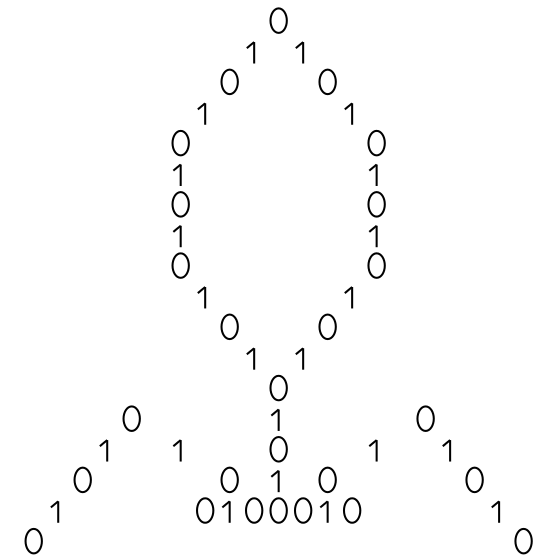
\includegraphics[scale=0.09]{images/fudepan.png}\\
            \vfill
            \begin{scriptsize}
                \textsc{FuDePAN} \\
            \end{scriptsize}
            \begin{tiny}
                \textsc{Fundación para el Desarrollo de la Programación en Ácidos Nucleicos} \\[1cm]
            \end{tiny}
        \end{center}
    \end{minipage}
}

\date{8 de Noviembre de 2013}

%--------------------------indice o temario
\begin{document}
   \frame{\titlepage}

    \frame{
    \frametitle{Temario:}
    \begin{footnotesize}\tableofcontents\end{footnotesize}
    }

%--------------------------secciones
\section{Introducción}

\subsection{FuDePAN}
	\begin{frame}{\textbf{FuDePAN}}
  	  \par La \textbf{Fu}ndación para el \textbf{De}sarrollo de la \textbf{P}rogramación en \textbf{Á}cidos \textbf{N}ucleicos es una ONG (organización no gubernamental) concebida	para fomentar el desarrollo de técnicas y tecnologías para la Programación en Ácidos Nucleicos, al servicio de la salud humana.\\[0.2cm]

	  \pause
  	  \begin{itemize}
      	\item Fundada en 2006.
      	\item Bioinformática ingenieril.
      	\item I+D.
      	\item Colaboran
      	  \begin{itemize}
      	      \item Estudiantes: Voluntarios y tesistas
      	      \item Profesionales: Ámbito industrial y académico.
      	  \end{itemize}
      	\item Todo lo desarrollado por la fundación se encuentra bajo GPLv3.
      \end{itemize}	
	\end{frame}

    \begin{frame}{\textbf{FuDePAN (cont.)}}
       \large{\textbf{Pilares}}
       \begin{center}
           
\includegraphics[scale=0.30]{images/fudesuma.png}
       \end{center}
       \pause
       \begin{block}{Naturaleza de los problemas}
           \begin{itemize}
               \item Corren mucho tiempo
               \item Alta performance
               \item Resultados impactan en nuevos problemas y personas.
           \end{itemize}
      \end{block}
	\end{frame}

\subsection{Motivación}
  \begin{frame}\frametitle{\textbf{Motivación}}      
    \begin{itemize}
      \item \textbf{Dado a que:}
        FuDePAN tenía un trabajo disponible.
      \item \textbf{Surgió la necesidad de:}
        Investigar y desarrollar un software.
      \item \textbf{Objetivo Principal:}
        contrastar una teoría (una hipótesis).
    \end{itemize}

    \begin{minipage}{3cm \textwidth}
       \begin{block}{\small{Dr. Daniel Rabinovich}}
        \hspace*{.25cm}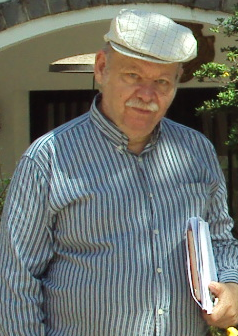
\includegraphics[scale=.25]{images/danielR.png}        
        \vskip .1cm
        \hspace*{.9cm}
\includegraphics[scale=.25]{images/inbird.jpg}
      \end{block}      
    \end{minipage}
    \begin{minipage}{6cm}
      \begin{center}
        \pause
        \textbf{Perspectiva Personal}
        \begin{itemize}
          \item Tarea desafiante.
          \item Integrarse en un grupo de desarrollo formado.
          \item Adaptarse a nuevos entornos.
          \item Contribuir a la salud.
          \item Retribuir con trabajo.
        \end{itemize}
      \end{center}
    \end{minipage}       
    
  \end{frame}
\section{Marco Teórico}
  \subsection{Conceptos de Biología}

    \begin{frame}\frametitle{\textbf{Conceptos de Biología}}
    \end{frame}
    \begin{frame}\frametitle{\textbf{Conceptos de Biología}}
        \begin{center}
          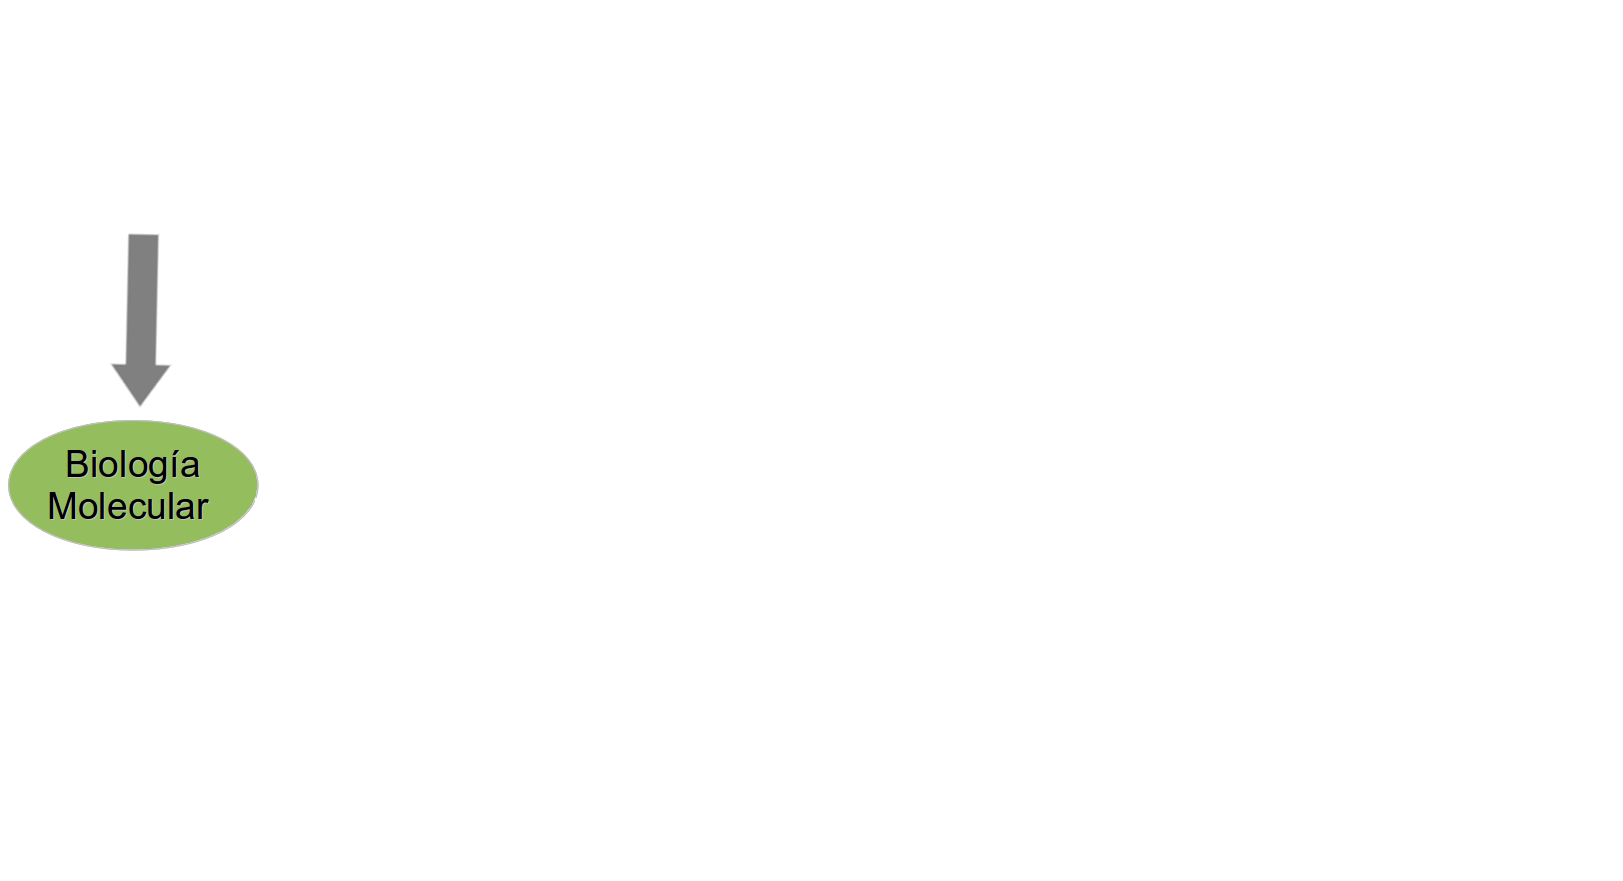
\includegraphics[scale=.2]{images/biologia1.png}
        \end{center}
    \end{frame}

    \begin{frame}\frametitle{\textbf{Conceptos de Biología}}
        \begin{center}
          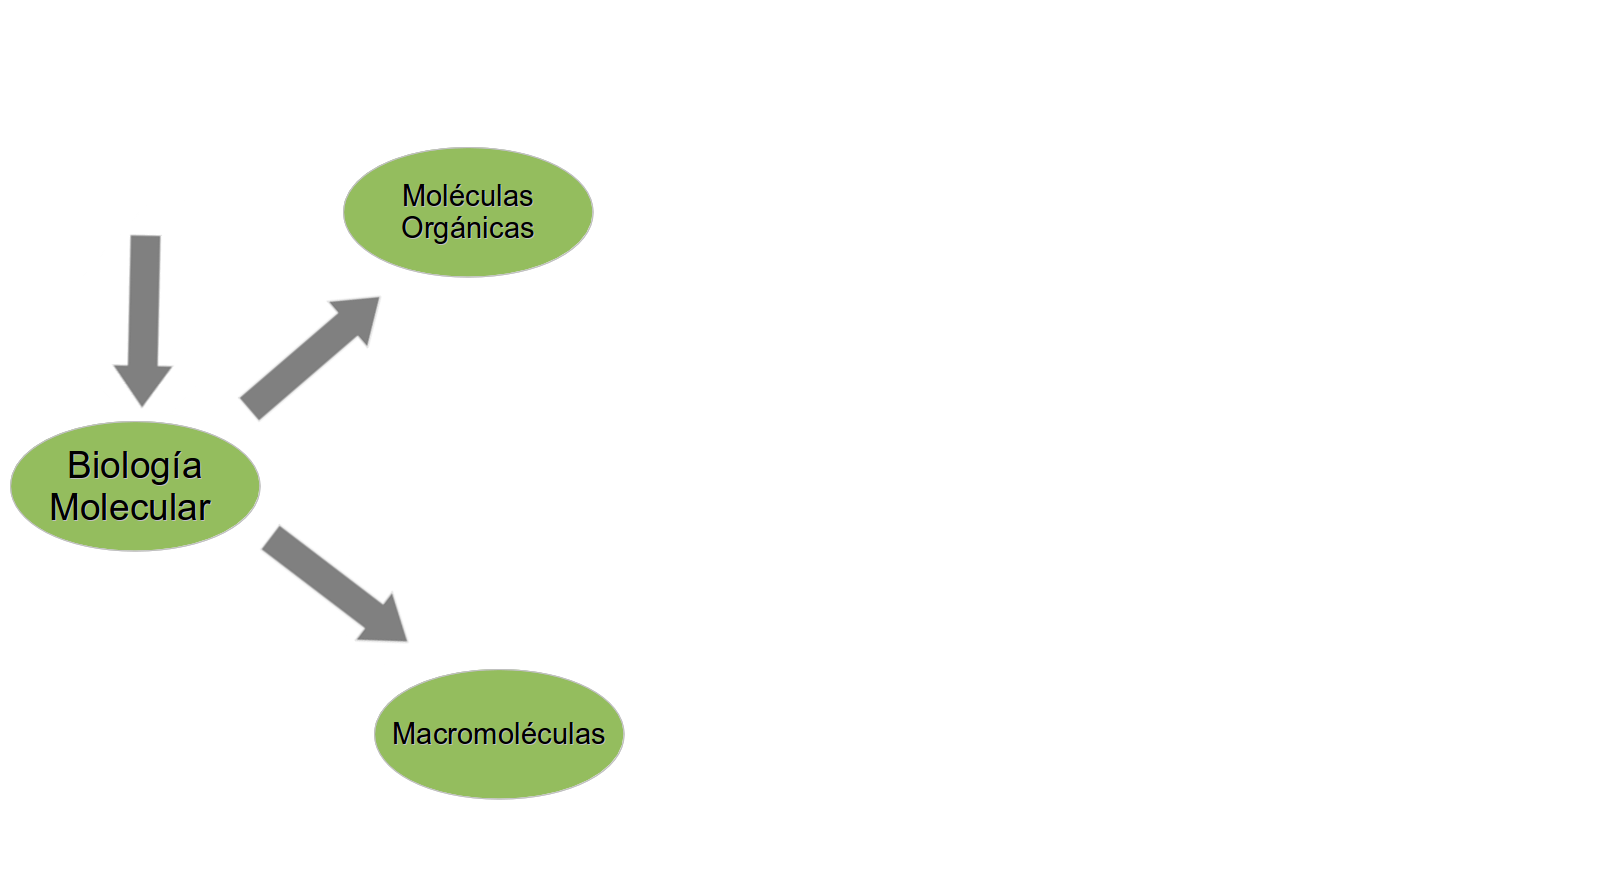
\includegraphics[scale=.2]{images/biologia2.png}
        \end{center}
    \end{frame}

    \begin{frame}\frametitle{\textbf{Conceptos de Biología}}
        \begin{center}
          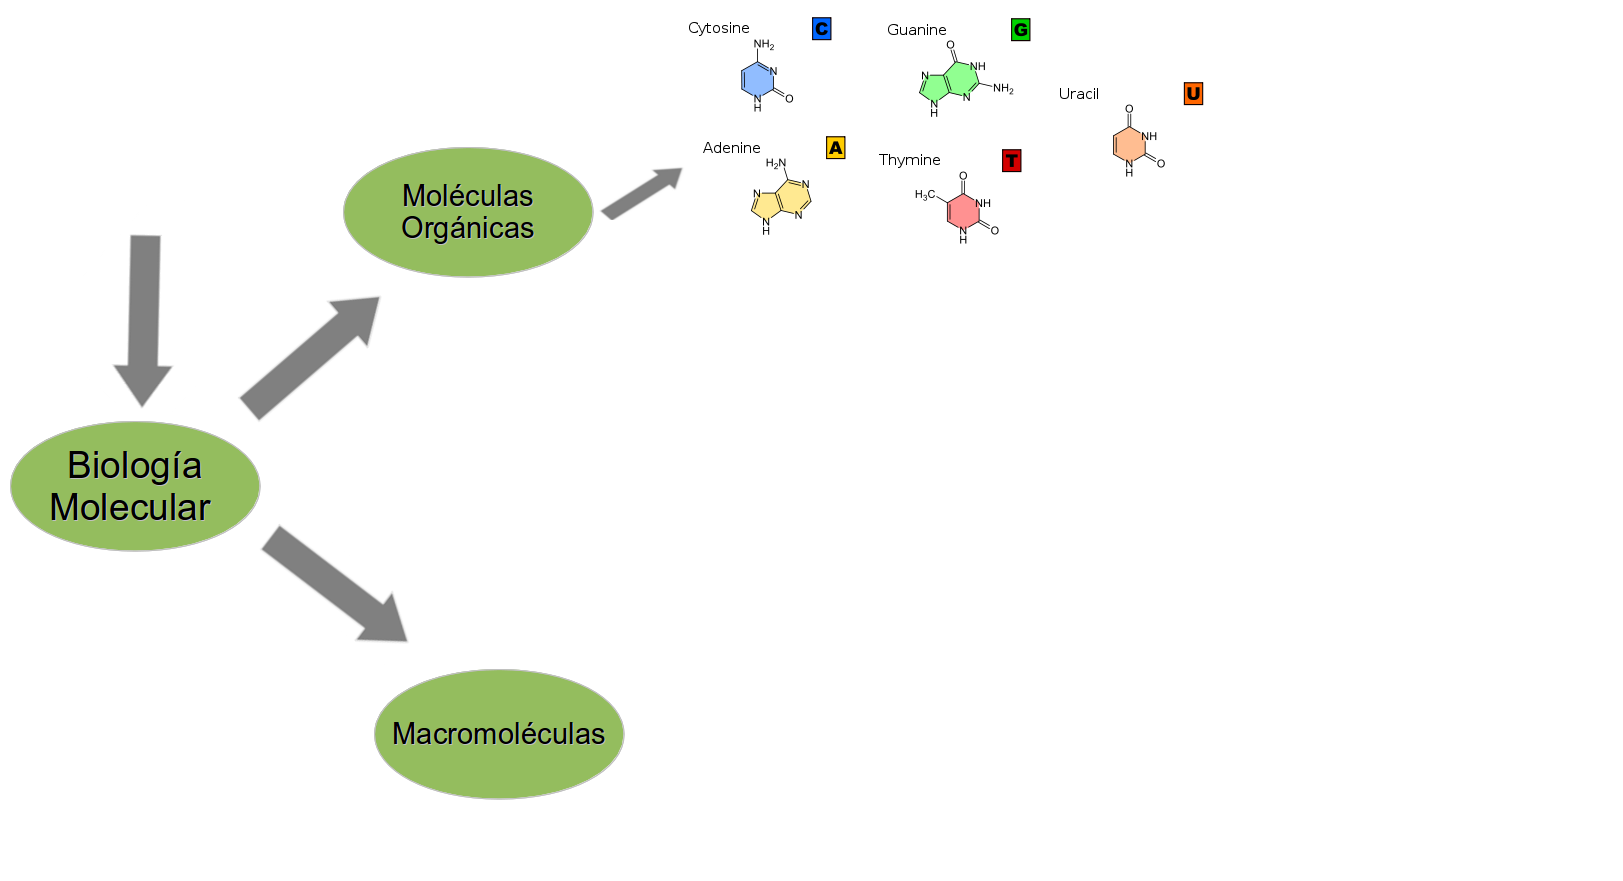
\includegraphics[scale=.2]{images/biologia3.png}
        \end{center}
    \end{frame}
    
    \begin{frame}\frametitle{\textbf{Conceptos de Biología}}
        \begin{center}
          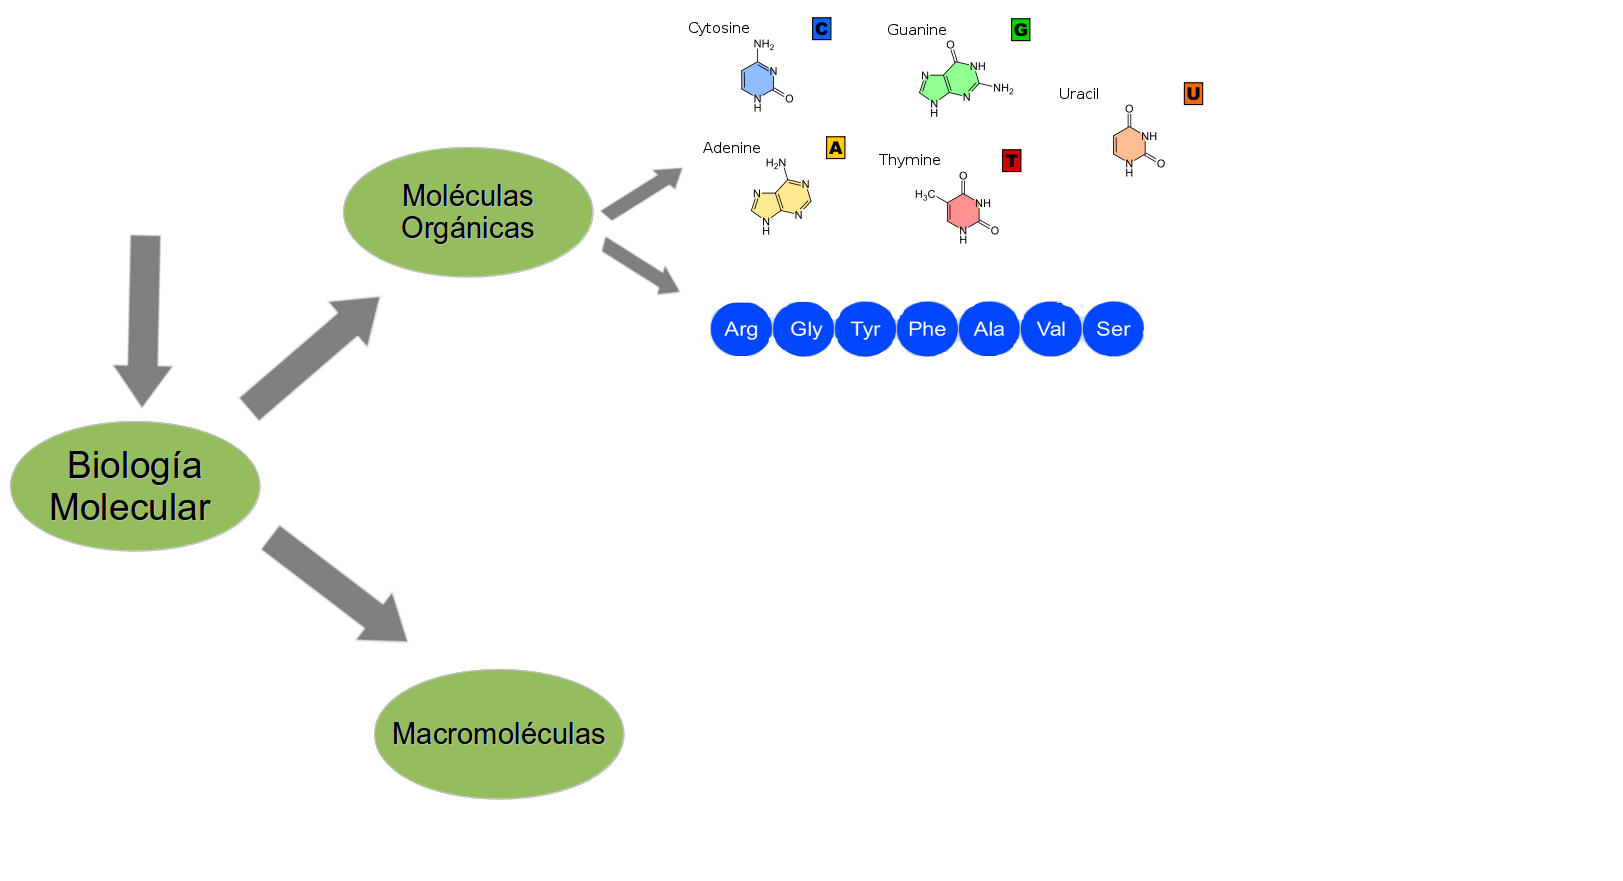
\includegraphics[scale=.2]{images/biologia4.png}
        \end{center}
    \end{frame}

    \begin{frame}\frametitle{\textbf{Conceptos de Biología}}
        \begin{center}
          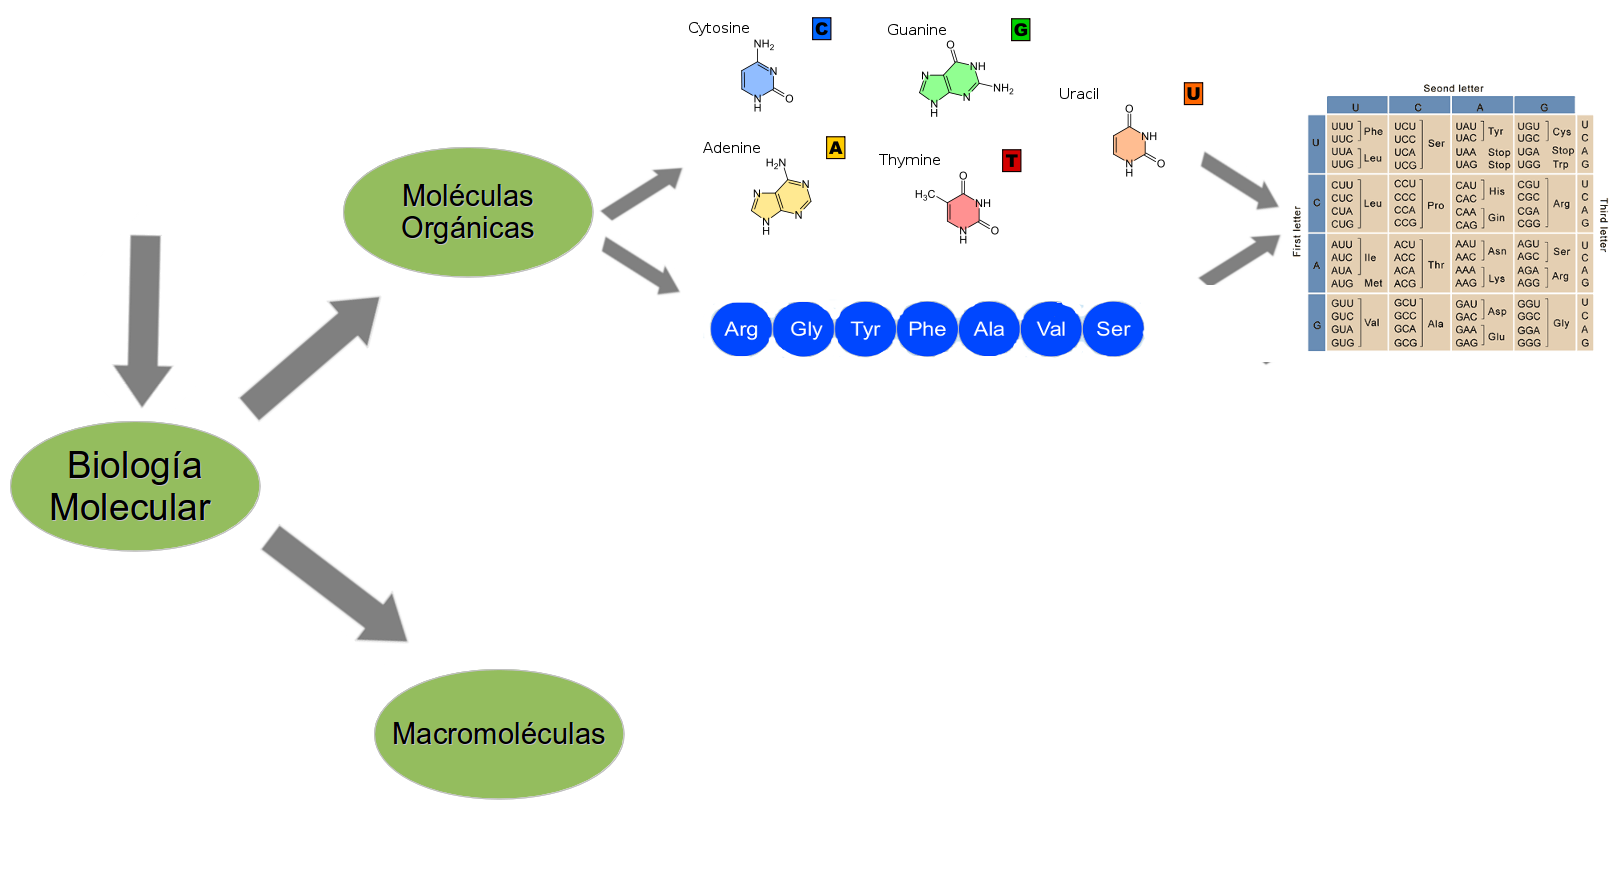
\includegraphics[scale=.2]{images/biologia5.png}
        \end{center}
    \end{frame}

    \begin{frame}\frametitle{\textbf{Conceptos de Biología}}  
        \begin{center}
          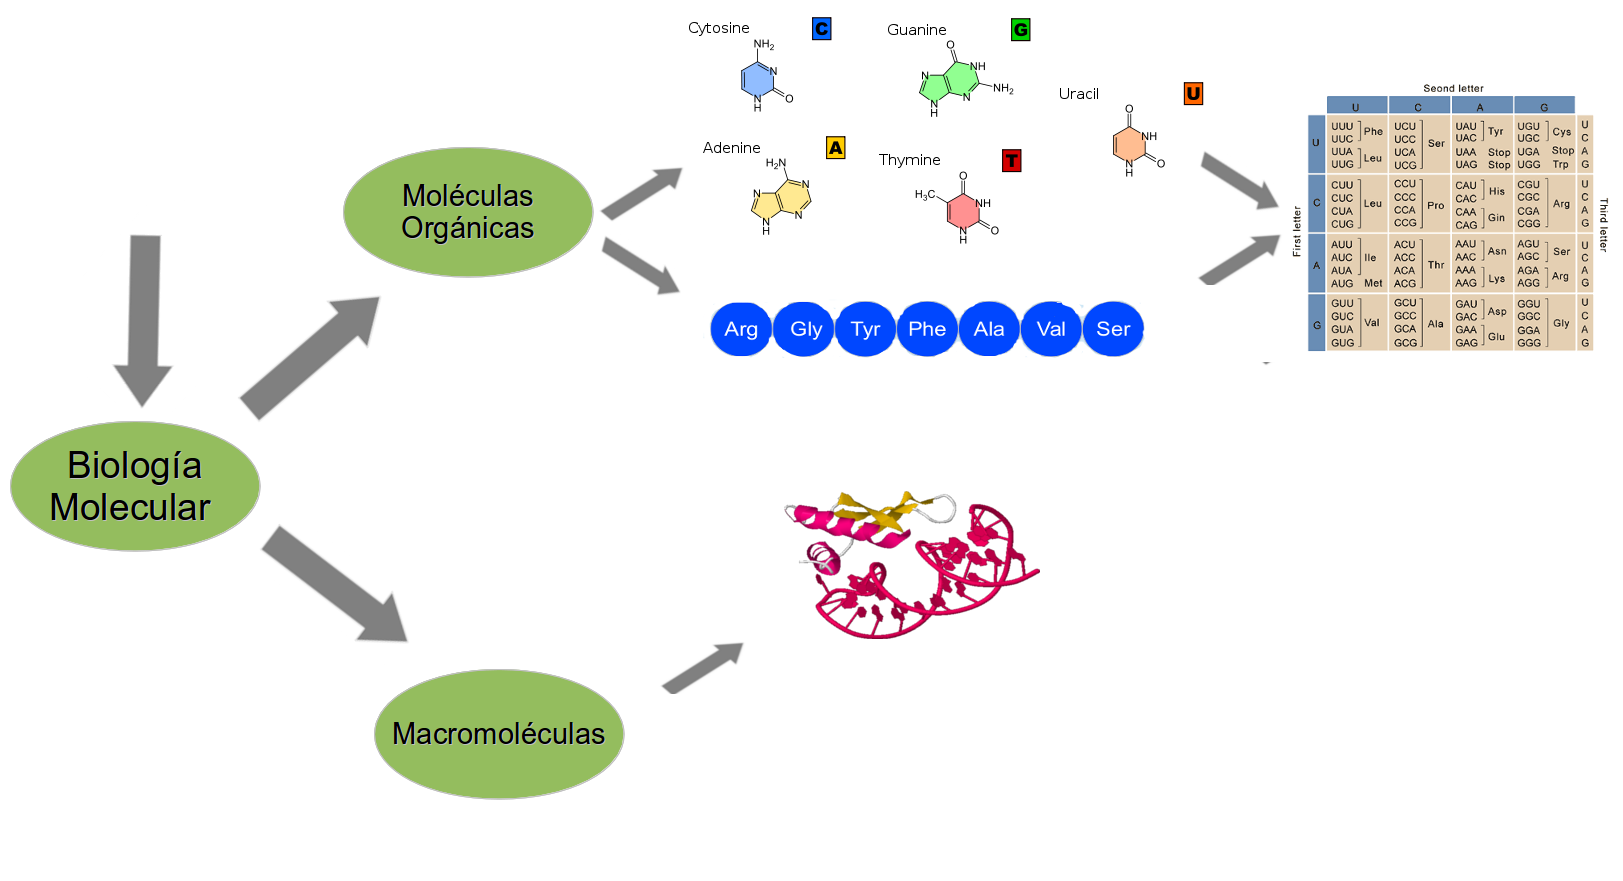
\includegraphics[scale=.2]{images/biologia6.png}
        \end{center}
    \end{frame}

    \begin{frame}\frametitle{\textbf{Conceptos de Biología}}
        \begin{center}
          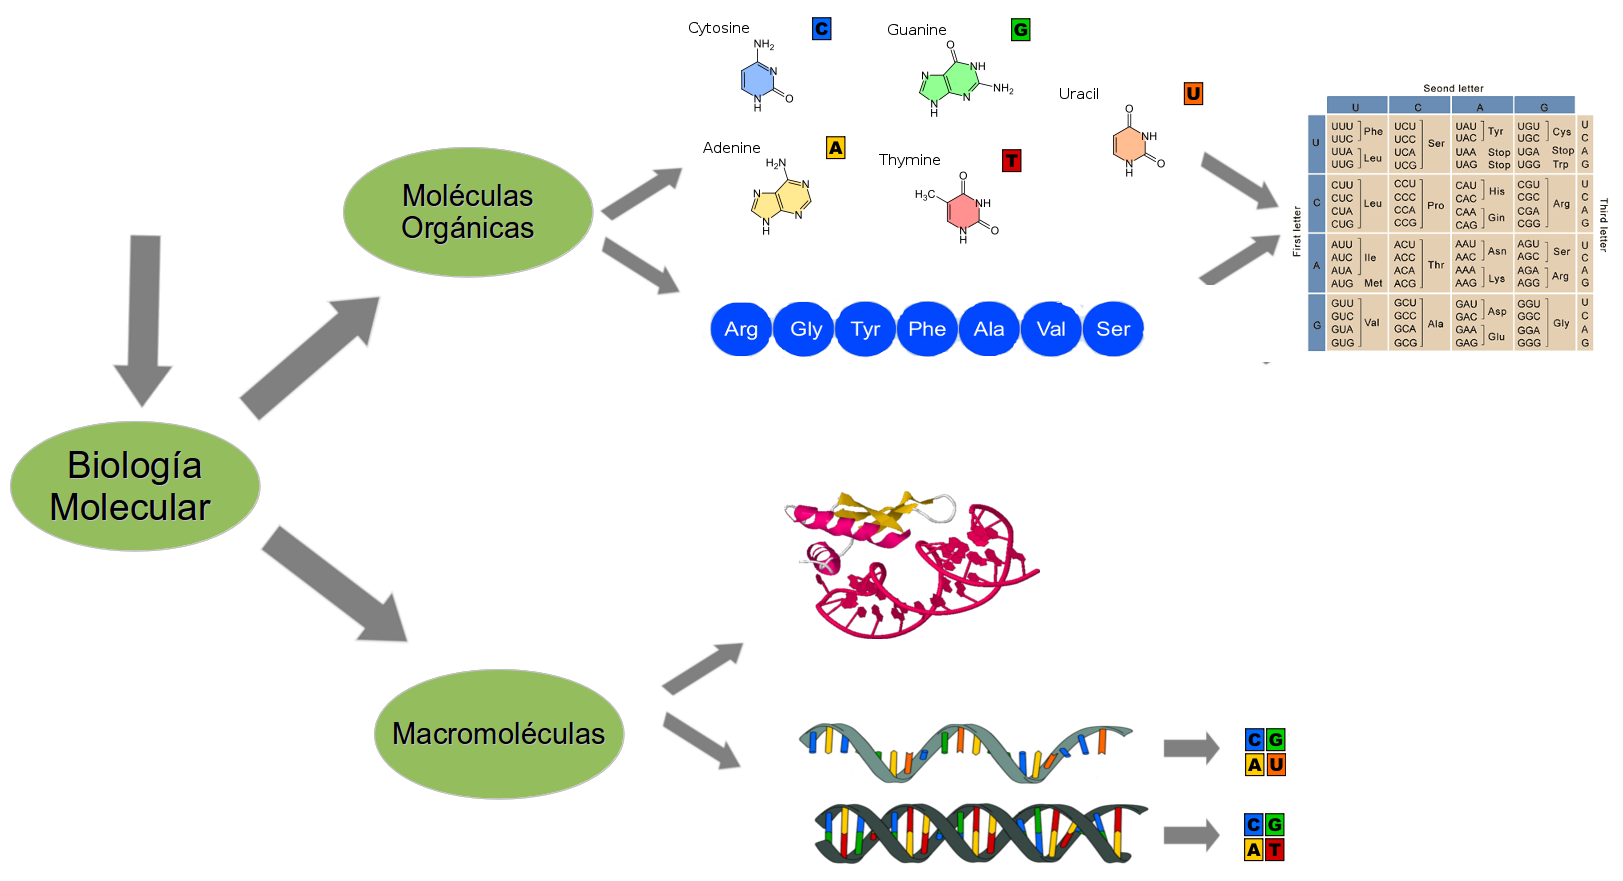
\includegraphics[scale=.2]{images/biologia7.png}
        \end{center}
    \end{frame}

    \begin{frame}\frametitle{\textbf{Ácidos Nucleícos}}
      \begin{block}{}
        \begin{center}
          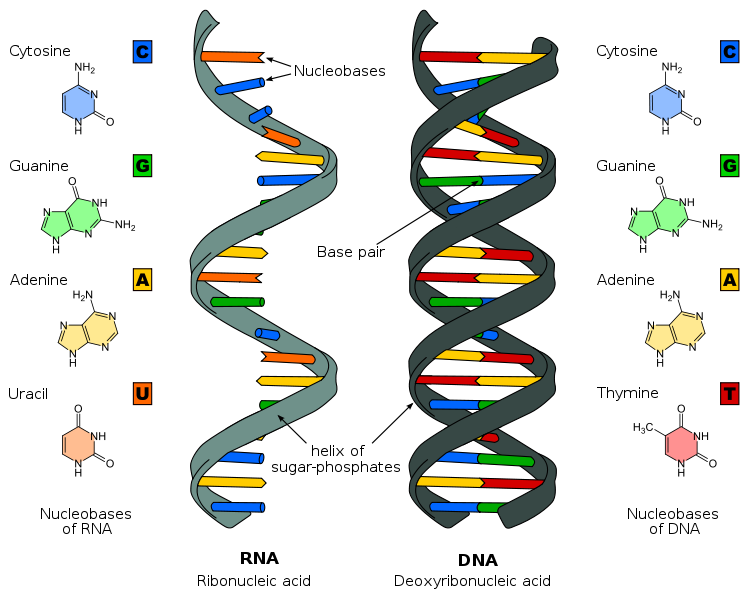
\includegraphics[scale=.3]{images/adnrna.png}
        \end{center}
      \end{block}
    \end{frame}

    \begin{frame}\frametitle{\textbf{Ácidos Nucleícos (cont.)}}
      \begin{block}{RNA}
        \begin{figure}[h]
          \begin{minipage}{0.7 \textwidth} 
            Generalmente, consiste en una hebra de cadena simple, la cual usualmente es trascripta a partir de una porci\'on de ADN y se utiliza posteriormente en la c\'elula para la s\'intesis de prote\'inas. Algunos virus poseen ARN como \'unico material gen\'etico cuya monohebra puede plegarse, dando lugar a lo que se conoce como estructura secundaria.
          \end{minipage}
          \begin{minipage}{3cm}
          \begin{center}
           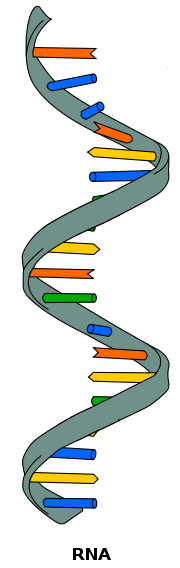
\includegraphics[scale=.15]{images/rna.png}
          \end{center}
          \end{minipage}
        \end{figure}
      \end{block}

      \begin{block}{La Estructura Primaria y Secundaria del RNA}
        La estructura primaria del ARN, es una secuencia de nucle\'otidos de longitud $n$, $A=a_{1}a_{2}a_{3}\dots a_{n}$ con $a_{i} \in \left\lbrace A, U, G, C \right\rbrace$. El plegamiento de una secuencia de ARN entre sus bases complementarias determina lo que se denomina estructura secundaria de ARN.
      \end{block}
    \end{frame}

    \begin{frame}\frametitle{\textbf{Estructura Secundaria del RNA (motifs)}}
        \begin{center}
          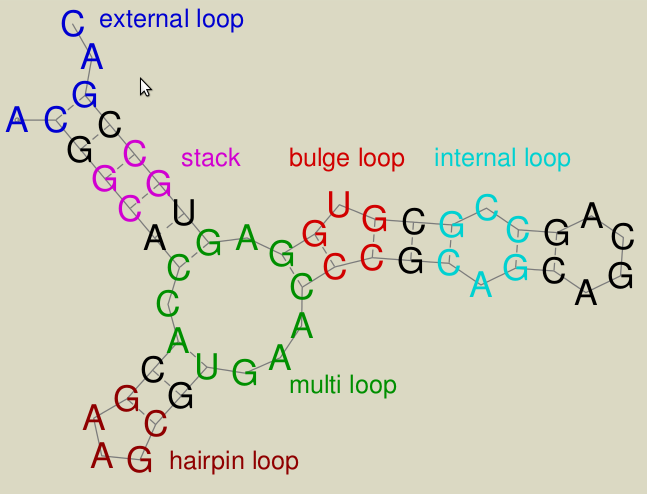
\includegraphics[scale=.38]{images/rnaMotifs.png}
        \end{center}       
    \end{frame}

    \begin{frame}\frametitle{\textbf{Estructura Secundaria del RNA (cont.)}}
        \begin{center}
          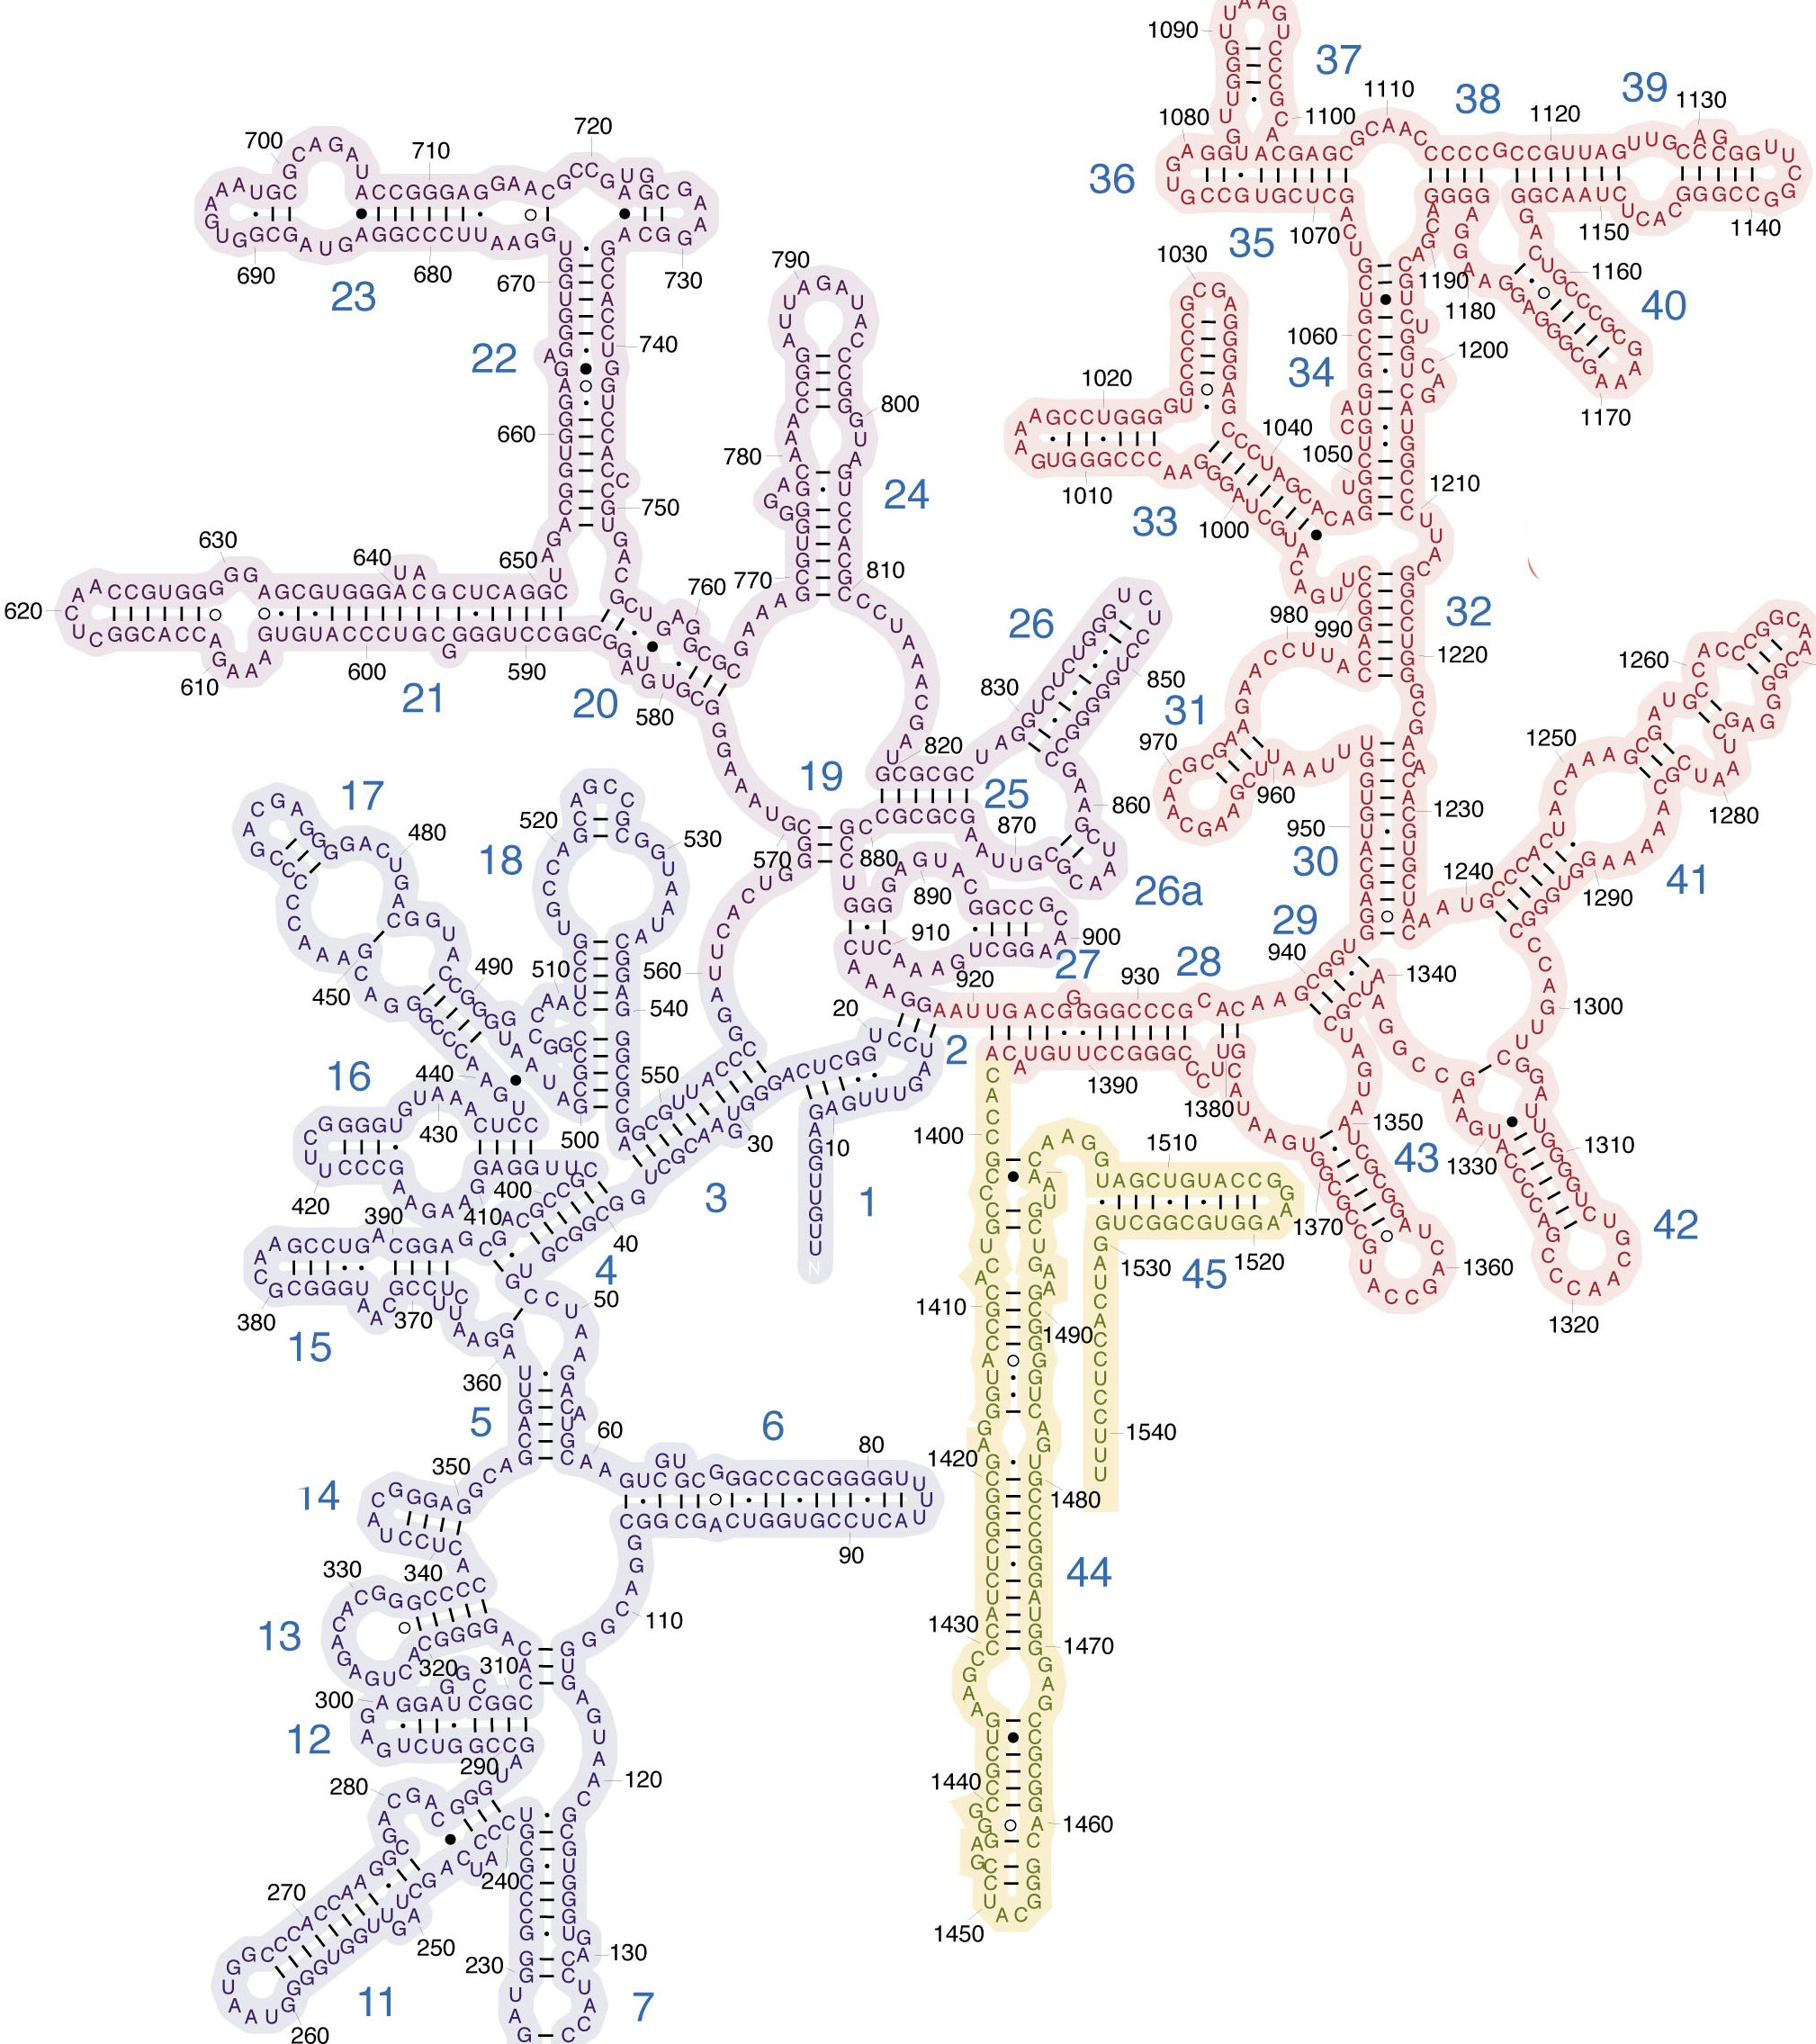
\includegraphics[scale=.39, angle=90]{images/complex.jpg}
        \end{center}       
    \end{frame}

    \begin{frame}\frametitle{\textbf{Dogma Central de la Biología}}
        \begin{center}
          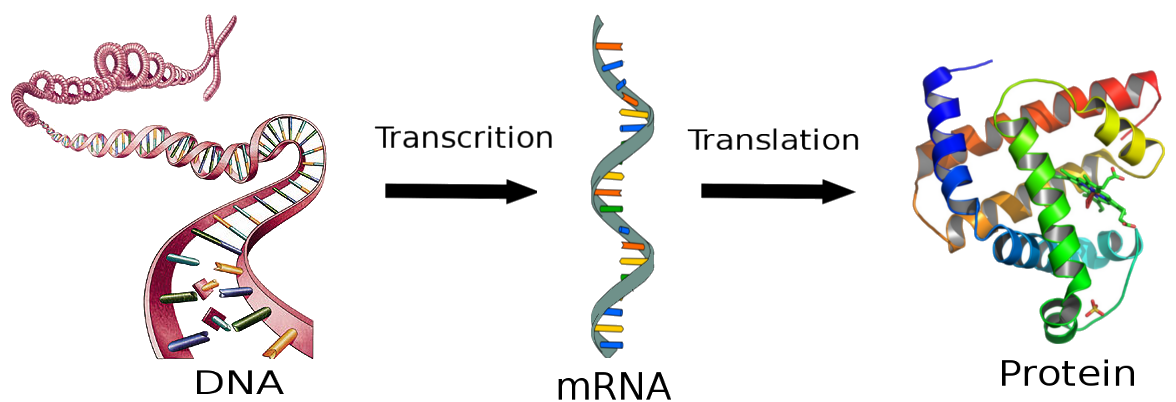
\includegraphics[scale=.26]{images/centralDogma.png}
        \end{center}       
    \end{frame}

\section{Descripción del Problema}
    \begin{frame}\frametitle{\textbf{Descripción del Problema}}
       \begin{block}{Hechos importantes:}
          \begin{minipage}{6cm\textwidth}
             \begin{itemize}
               \item Código genético degenerado.
               \item Codones Sinónimos.
               \item Uso de codones universal.
               \item Divergencia de codones no esclarificada.
             \end{itemize}  
           \end{minipage}
           \begin{minipage}{4cm}
               \hspace*{.7cm}
\includegraphics[scale=.35]{images/codonesSinonimos.png}
           \end{minipage}            
       \end{block}

       \pause
       \begin{block}{Hipótesis}
         \par \textbf{``La divergencia en el uso de codones sinónimos entre virus y huésped contribuye a disminuir la interferencia de los $_m$$_i$RNA en la expresión de los RNA mensajeros de origen viral."}
     \end{block}
    \end{frame}
    

\section{R-emo}
  \subsection{Metodología de Desarrollo}
      \begin{frame}\frametitle{\textbf{Metodología de Desarrollo}}
          \begin{center}
            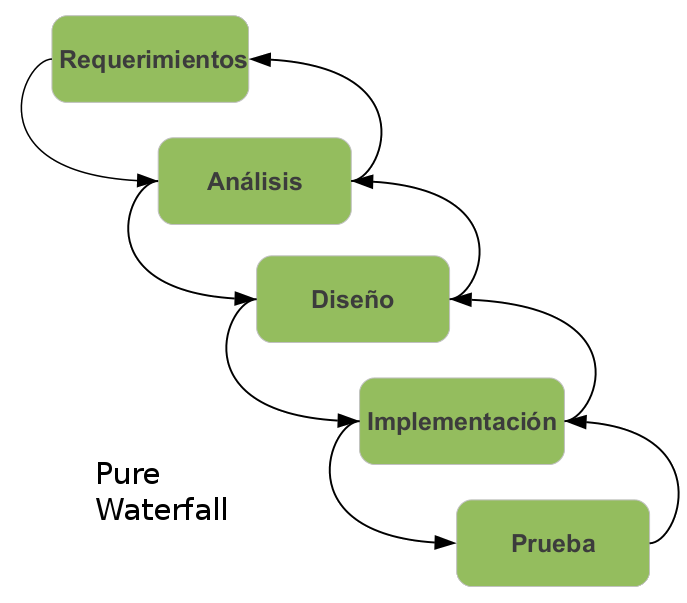
\includegraphics[scale=.4]{images/cascadaPuro.png}
          \end{center}
      \end{frame}  
      
      \begin{frame}\frametitle{\textbf{Consideraciones sobre la Metodología}}
          \begin{center}  
            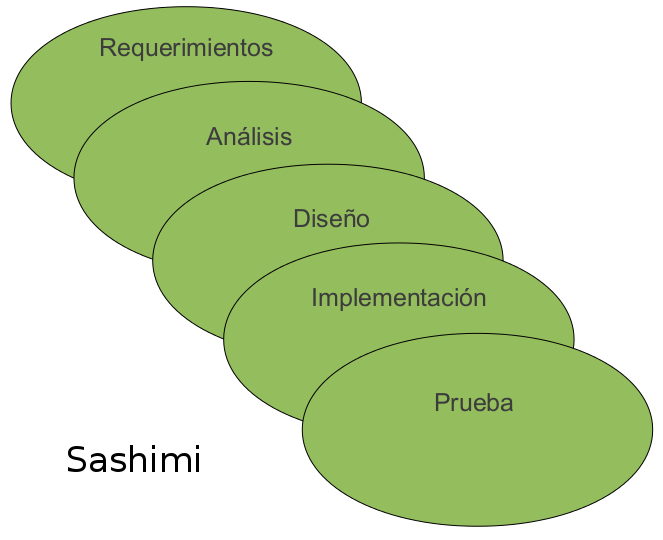
\includegraphics[scale=.42]{images/sashimi2.png}
          \end{center}
      \end{frame}  

      \begin{frame}\frametitle{\textbf{Consideraciones sobre la Metodología (cont.)}}        
          \begin{center}
            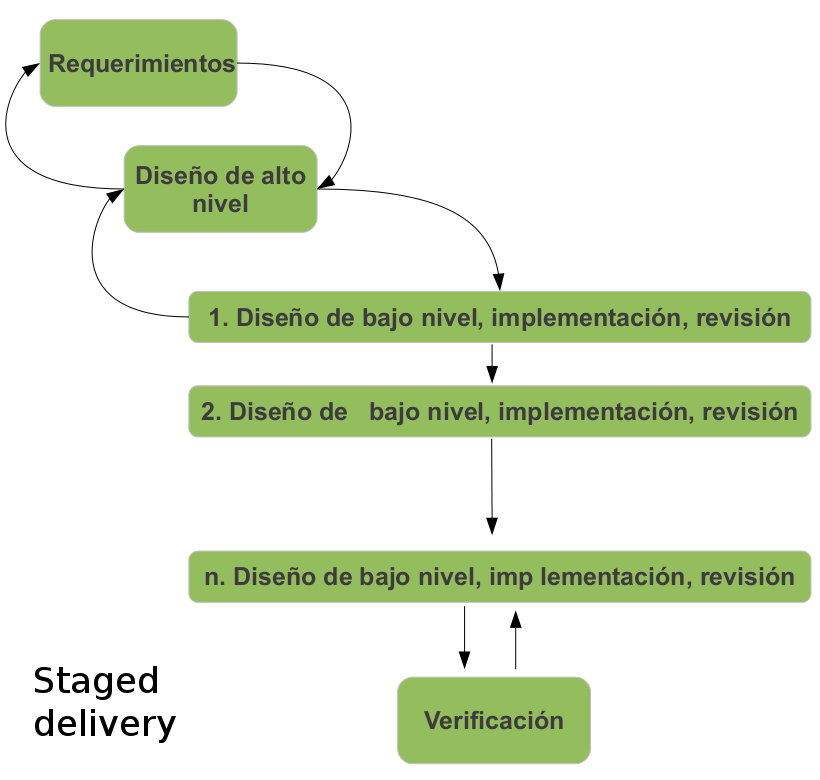
\includegraphics[scale=.35]{images/stagedDelivery2.png}
          \end{center}        
      \end{frame}  

  \subsection{Elicitación y Análisis}
      \begin{frame}\frametitle{\textbf{Especificación}}
        \hspace*{-1cm} 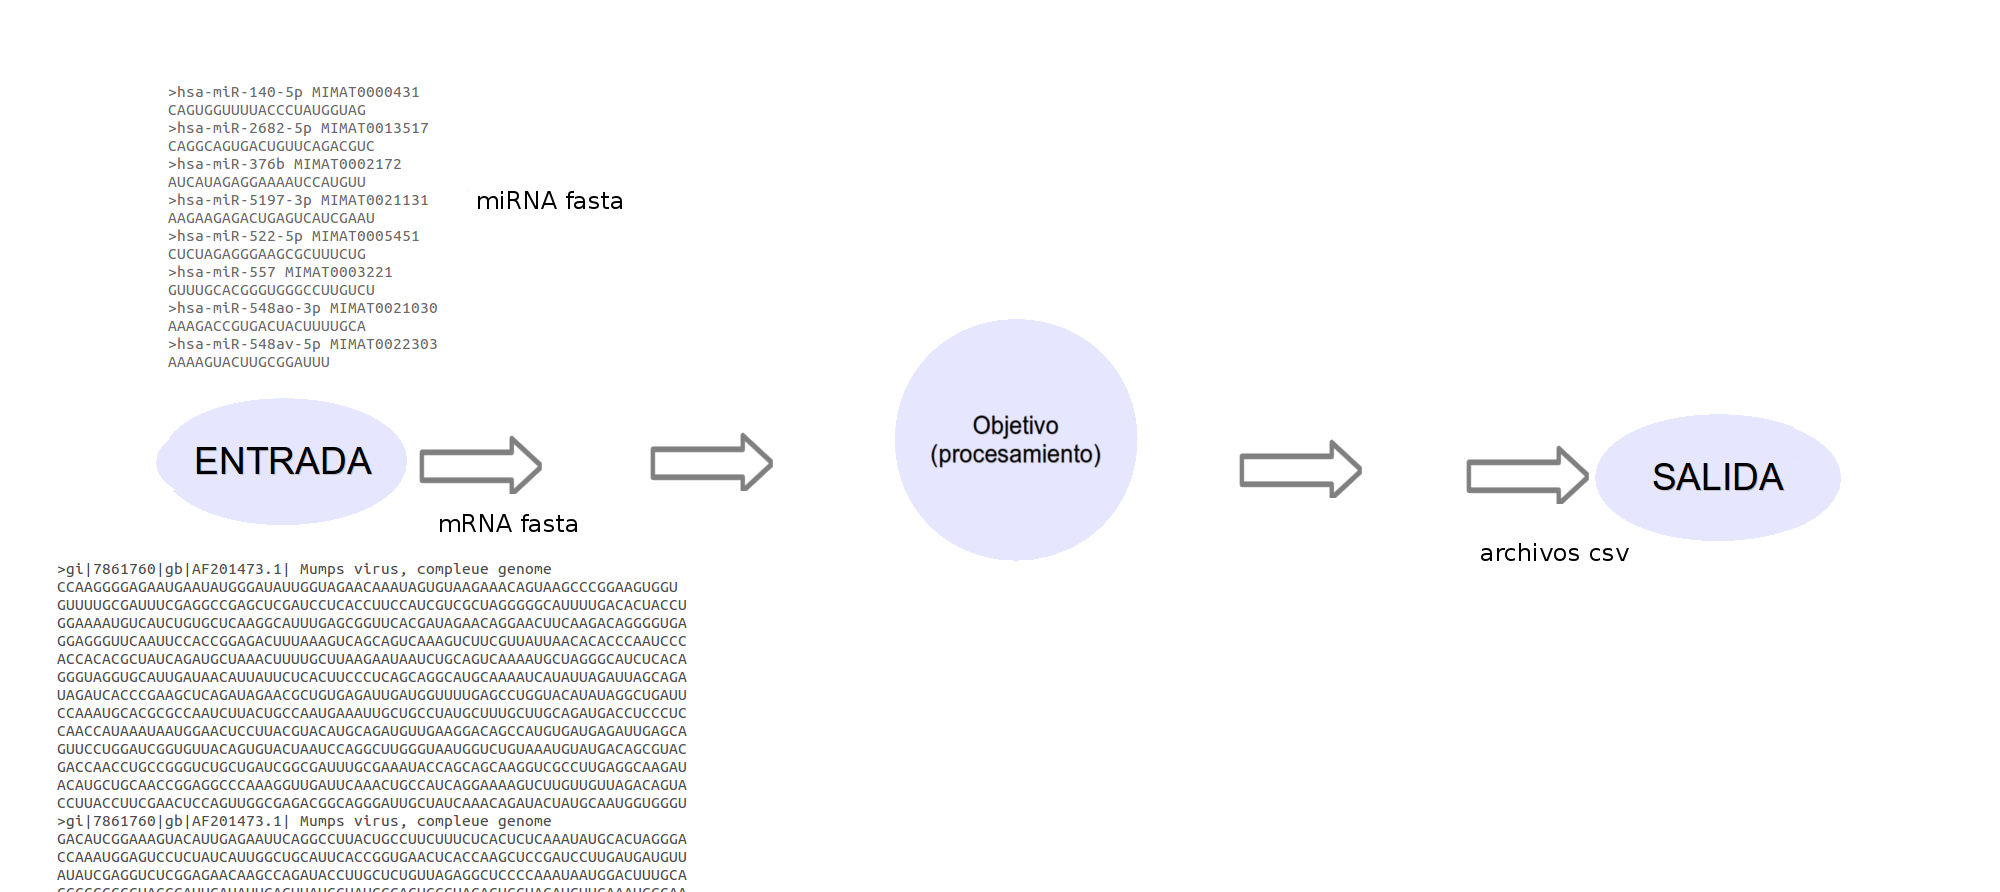
\includegraphics[scale=.19]{images/especificacion1.png}
      \end{frame}  

      \begin{frame}\frametitle{\textbf{Especificación (cont.)}}
        \hspace*{-.9cm}  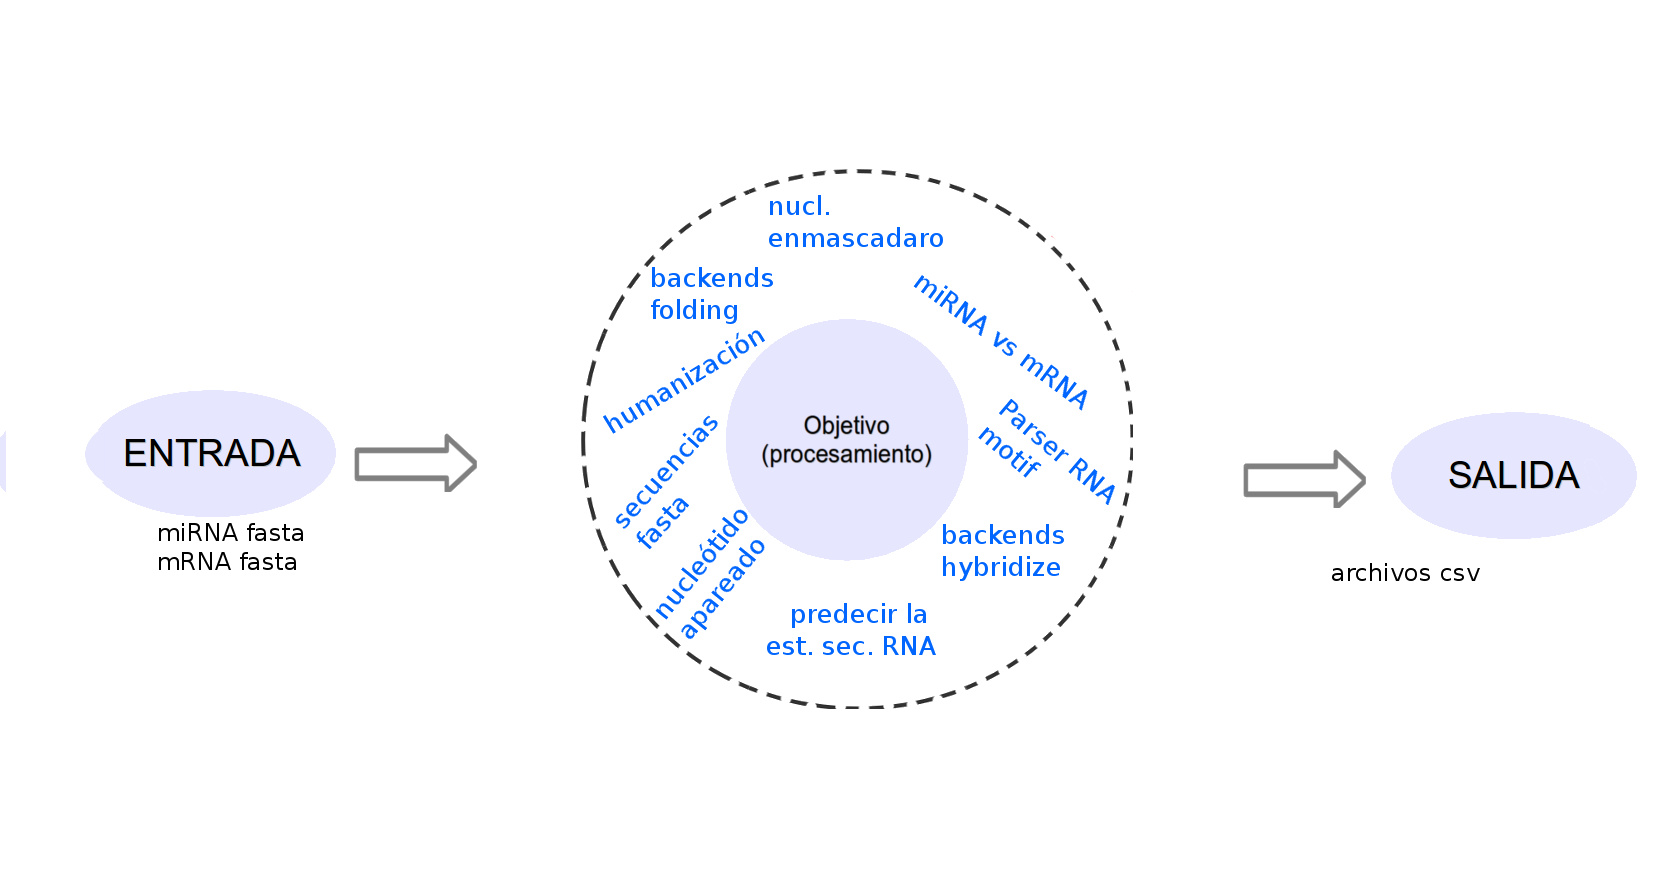
\includegraphics[scale=.2]{images/especificacion2.png}
      \end{frame}  

      \begin{frame}\frametitle{\textbf{Especificación (cont.)}}
        \hspace*{-.5cm} 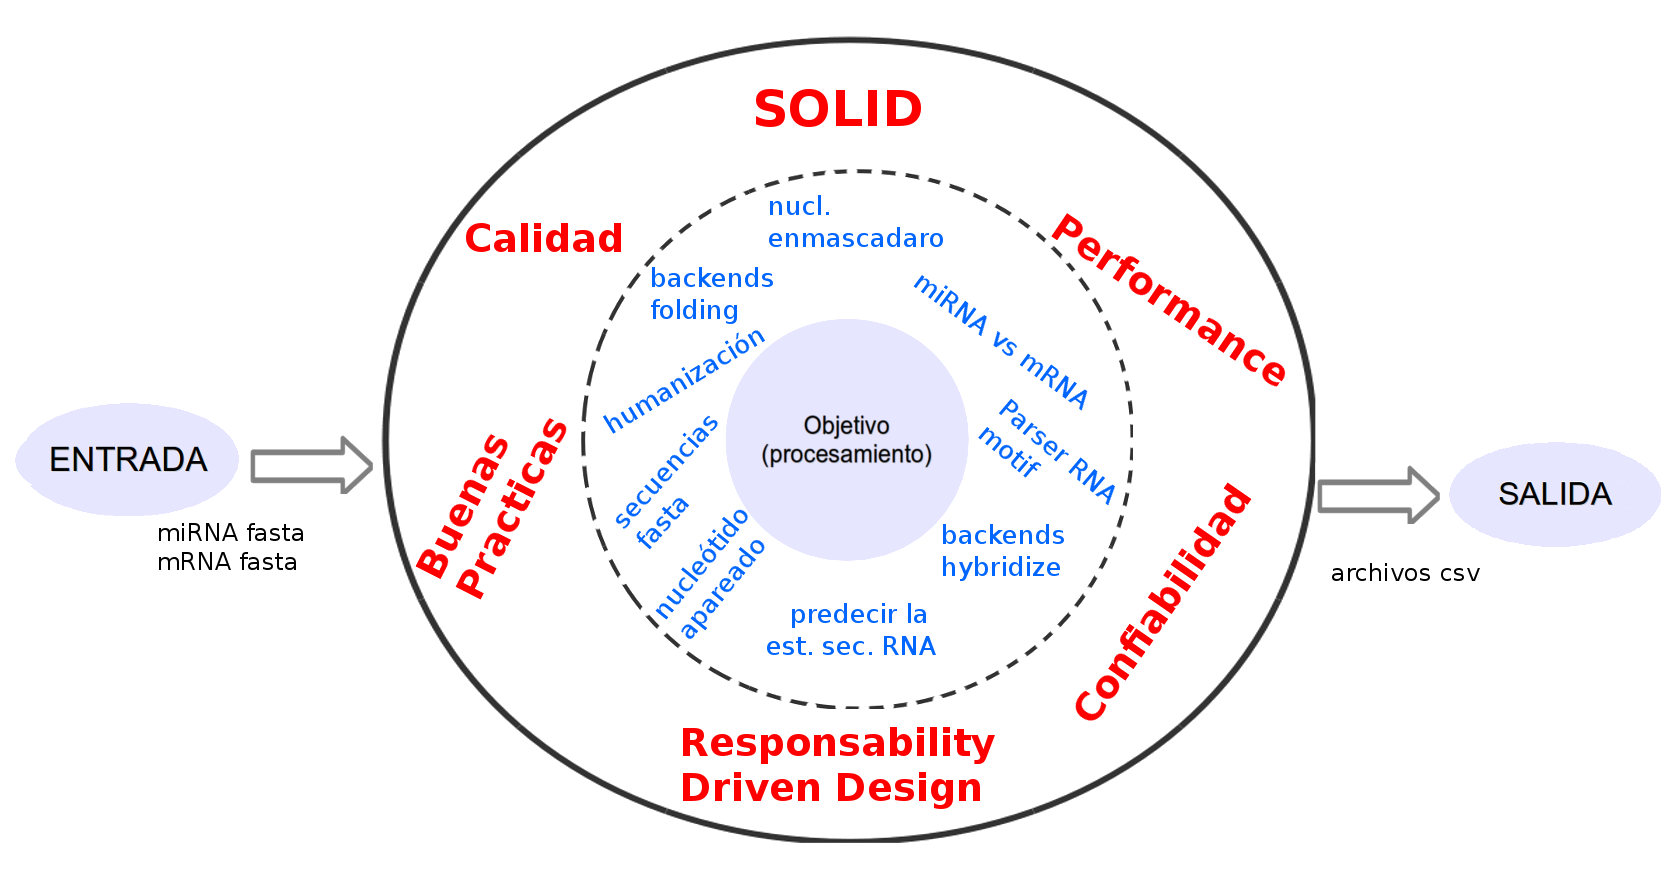
\includegraphics[scale=.2]{images/especificacion3.png}
      \end{frame}  

      \begin{frame}\frametitle{\textbf{Creación de librerías}}
        \begin{block}{Surgen:}
          \begin{itemize}
            \item \textbf{fideo   :} Folding Interface Dynamic Exchange Operations
                \vskip .05cm
                \hspace*{2.9cm}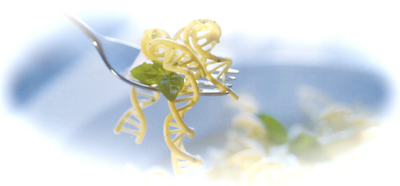
\includegraphics[scale=.2]{images/fideo.png}
            \item \textbf{acuoso  :} Abstract Codon Usage Optimization Software for Organisms
                \vskip .05cm
                \hspace*{3.5cm}
\includegraphics[scale=.3]{images/acuoso.png}
            \item \textbf{etilico :} External Tools Invocation LIbrary and COmponent
                \vskip .05cm
                \hspace*{2.25cm}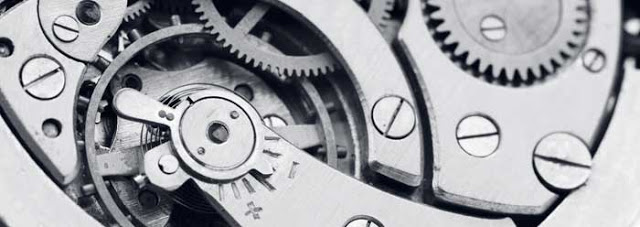
\includegraphics[scale=.19]{images/etilico.jpg}
          \end{itemize}  
        \end{block}  
      \end{frame}  

  \subsection{Diseño}
      \begin{frame}\frametitle{\textbf{Principios de Diseño}}
          \begin{block}{Resposability-Driven Design}
              \begin{minipage}{2cm \textwidth}
                  
\includegraphics[scale=.2]{images/manos.jpg}
              \end{minipage}
              \begin{minipage}{8cm}
                  \begin{itemize}
                    \item Que responsabilidades debe cubrir el sistema.
                    \item Cuales serán los objetos responsables de llevarlas a cabo.                    
                  \end{itemize}                  
              \end{minipage}           
          \end{block}  

      \begin{block}{SOLID}
      \begin{minipage}{7cm \textwidth}
          \begin{itemize}
            \item   \textbf{S}ingle Responsibility Principle (SRP)
            \item   \textbf{O}pen-Closed Principle (OCP)
            \item   \textbf{L}iskov Substitution Principle (LSP)
            \item   \textbf{I}nterface Segregation Principle (ISP)
            \item   \textbf{D}ependency Inversion Principle (DIP)          
          \end{itemize}            
    \end{minipage}
    \begin{minipage}{3cm}
      
\includegraphics[scale=.3]{images/solid.png}
    \end{minipage}     
    \end{block}         
      \end{frame}  

      \begin{frame}\frametitle{\textbf{Arquitectura}}
        \begin{center}
          %A un alto nivel de componentes
          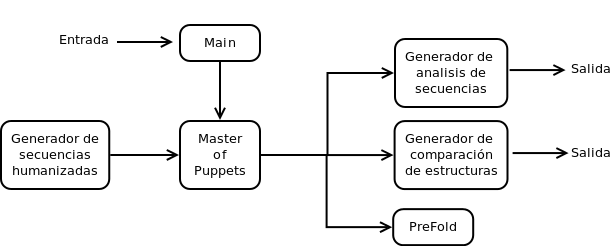
\includegraphics[scale=.4]{images/componenteRemo.png}
        \end{center}
      \end{frame}  

      \begin{frame}\frametitle{\textbf{Arquitectura (refinando)}}
        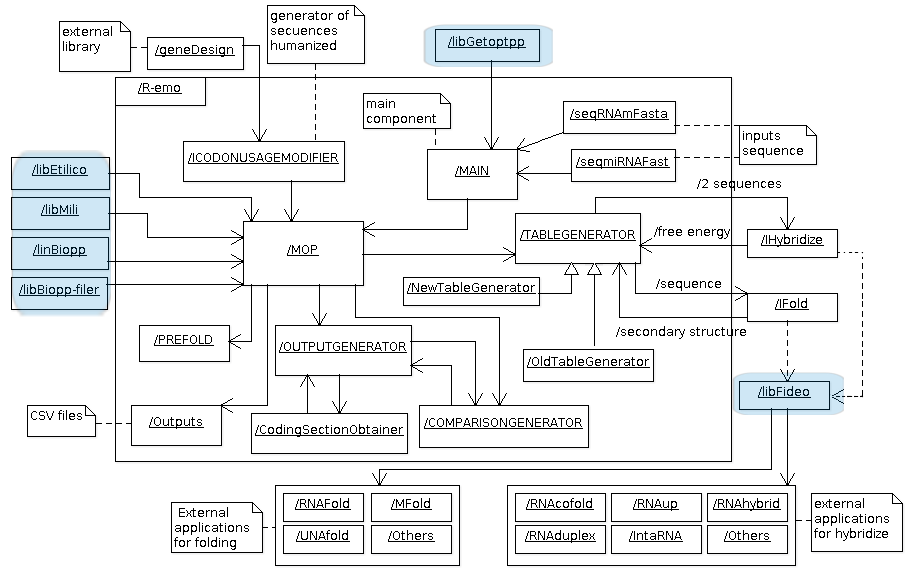
\includegraphics[scale=.35]{images/arquitectura.png}
      \end{frame}  

      \begin{frame}\frametitle{\textbf{Diagrama de Clases}}
        \begin{center}
          
\includegraphics[scale=.25]{images/emptyClass.png}
        \end{center}
      \end{frame}  

      \begin{frame}\frametitle{\textbf{Diagrama de Clases (Cont.)}}
        \begin{center}
          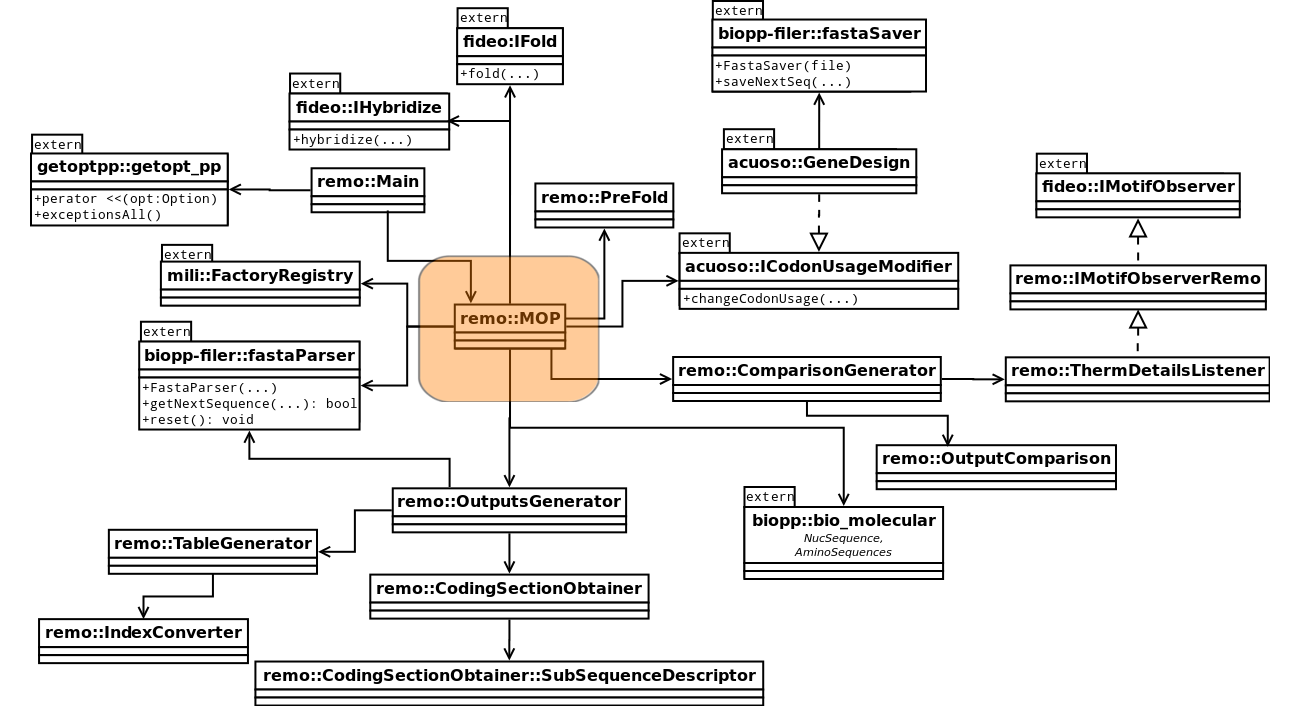
\includegraphics[scale=.25]{images/emptyClass2.png}
        \end{center}
      \end{frame}  

      \begin{frame}\frametitle{\textbf{Diagrama de Clases (Cont.)}}
        \begin{center}
          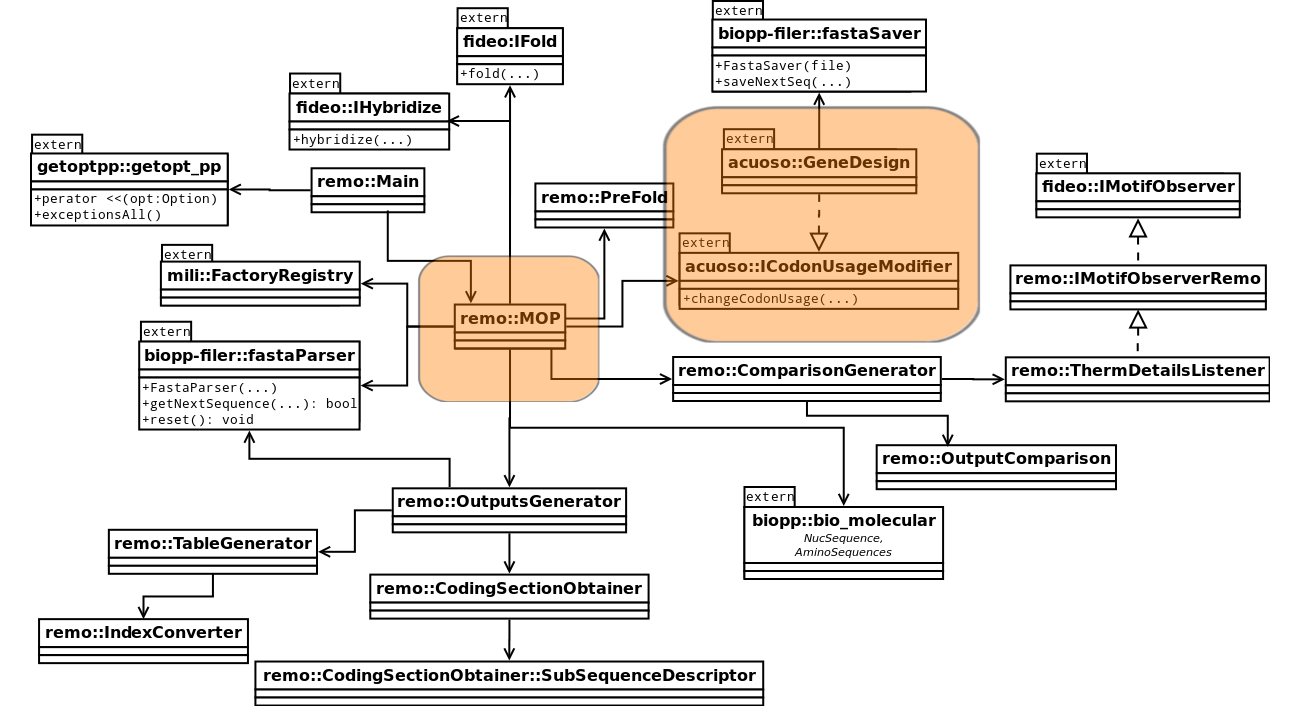
\includegraphics[scale=.25]{images/emptyClass3.png}
        \end{center}
      \end{frame}  

      \begin{frame}\frametitle{\textbf{Diagrama de Clases (Cont.)}}
        \begin{center}
          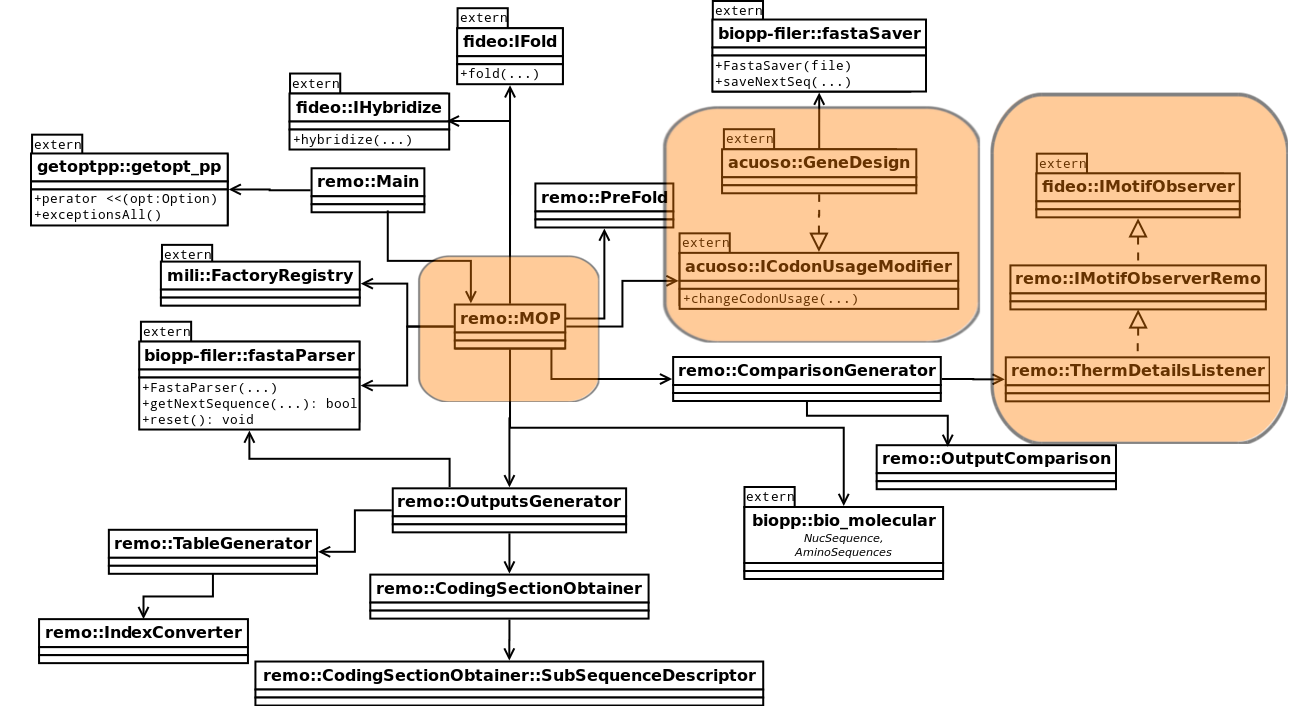
\includegraphics[scale=.25]{images/emptyClass4.png}
        \end{center}
      \end{frame}  

      \begin{frame}\frametitle{\textbf{Librerías Implementadas}}
        \begin{center}
          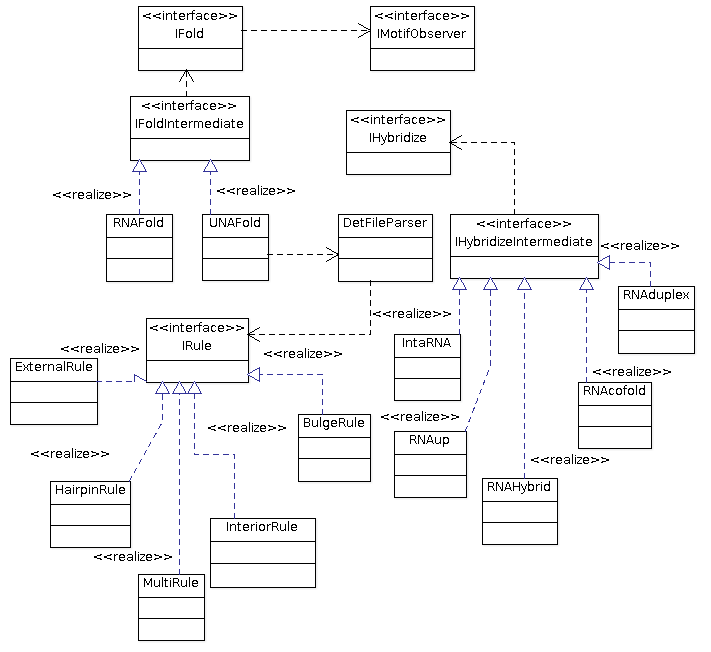
\includegraphics[scale=.3]{images/fideoInterface.png}
        \end{center}
      \end{frame}  

      \begin{frame}\frametitle{\textbf{Librerías Implementadas}}
        \begin{center}
           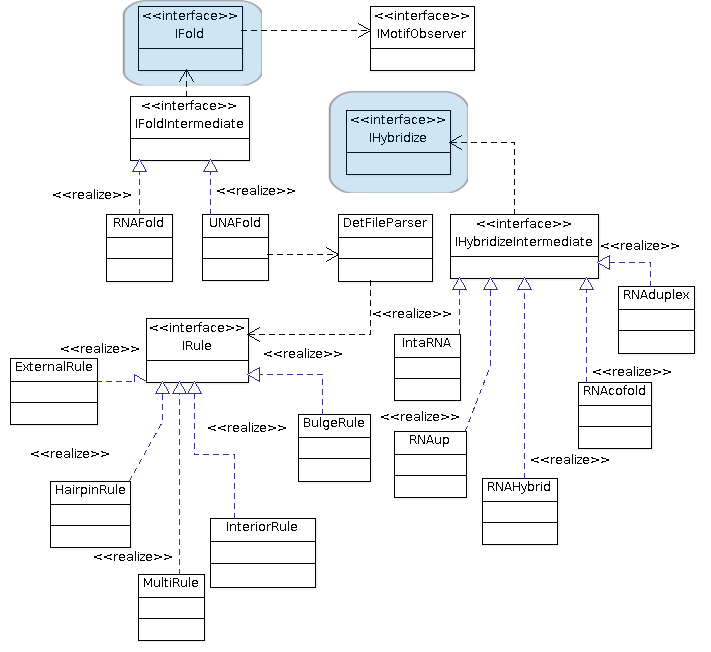
\includegraphics[scale=.3]{images/fideoInterface2.png}
        \end{center}
      \end{frame}

      \begin{frame}\frametitle{\textbf{Librerías Implementadas}}
        \begin{center}
          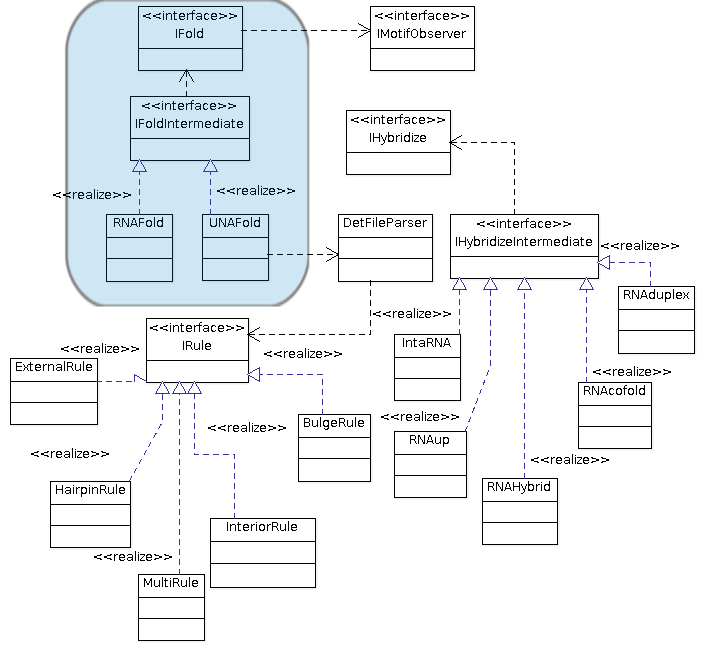
\includegraphics[scale=.3]{images/fideoInterface3.png}
        \end{center}
      \end{frame}

      \begin{frame}\frametitle{\textbf{Librerías Implementadas}}
        \begin{center}
          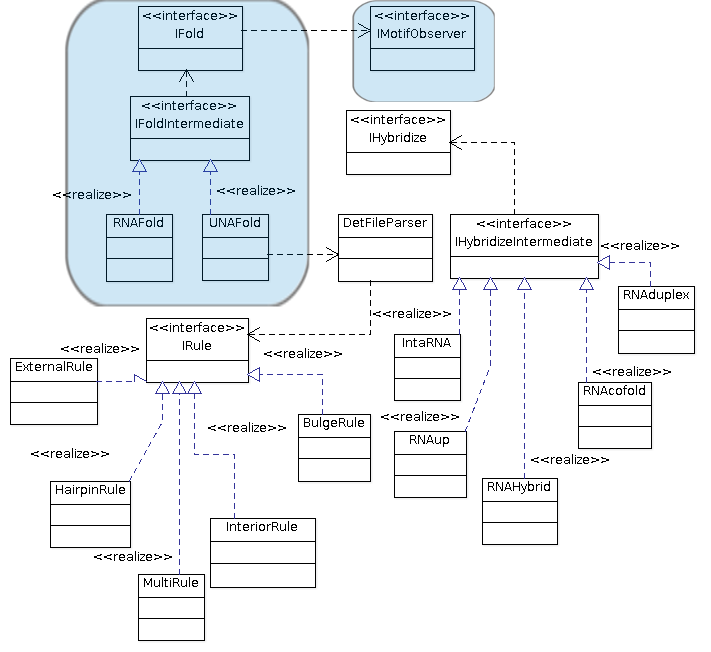
\includegraphics[scale=.3]{images/fideoInterface4.png}
        \end{center}
      \end{frame}

      \begin{frame}\frametitle{\textbf{Librerías Implementadas}}
        \begin{center}
          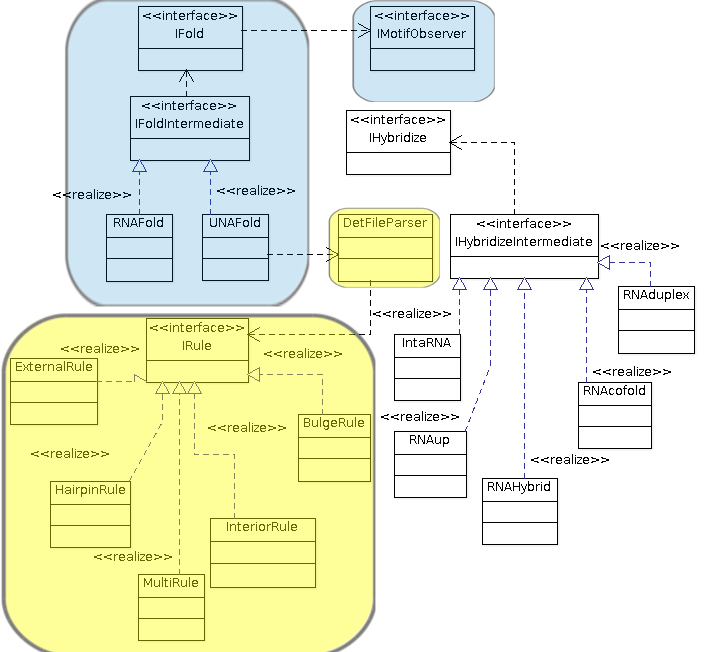
\includegraphics[scale=.3]{images/fideoInterface5.png}
        \end{center}
      \end{frame} 

  \subsection{Implementación} 
      \begin{frame}
        \frametitle{\textbf{Dependencias}}
        \begin{block}{Algunas de ellas son:}
          \begin{itemize}
            \item mili
            \item biopp 
            \item biopp-filer
            \item fud
          \end{itemize}  
        \end{block}          
        \hspace*{1.7cm}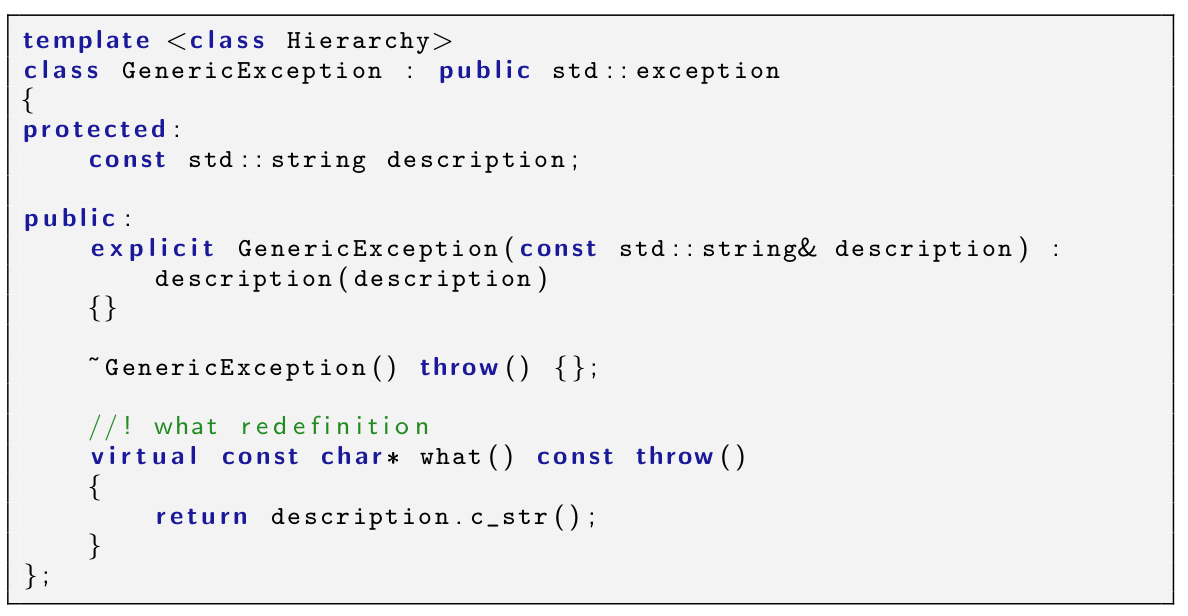
\includegraphics[scale=.18]{images/exampleMili.png}
      \end{frame}    
      
  \begin{frame}\frametitle{\textbf{Métricas de Código}}    
    \begin{table}[!htf]
    \rowcolors{2}{verde!20}{verde!5}
    \begin{tabular}{|l|r|r|r|r|c|}
    \hline
    \multicolumn{2}{|c|}{Files} & \multicolumn{3}{|c|}{Line Types} & \hspace{0.2cm}\% \\
    \hline
    \textbf{Type} & \textbf{Count} & \textbf{Blank} & \textbf{Comment} & \textbf{Source} & \small{\textbf{\#Comms./Tot.}}\\
    \hline
    \texttt{C++ source} & 10 & 161 & 553 & 1108 & 33.2 \\
    \hline
    \texttt{C++ header} & 11 & 150 & 757 & 273 & 73.4 \\
    \hline
    \textbf{Total}      & 21 & 311 & 1310 & 1381 & 48.6 \\
    \hline
    \end{tabular}    
    \end{table}
    \hspace*{3.5cm}Métricas CLOC para \textbf{Remo}.

    \begin{table}[!htf]
    % \begin{center}
    \rowcolors{2}{verde!20}{verde!5}
    \begin{tabular}{|l|r|r|r|r|c|}
    \hline
    \multicolumn{2}{|c|}{Files} & \multicolumn{3}{|c|}{Line Types} & \hspace{0.2cm}\% \\
    \hline
    \textbf{Type} & \textbf{Count} & \textbf{Blank} & \textbf{Comment} & \textbf{Source} & \small{\textbf{\#Comms./Tot.}}\\
    \hline
    \texttt{C++ source} & 10   &    161  &     344   &    967 & 26.2 \\
    \hline
    \texttt{C++ header} & 20   &    243  &    1222   &    603 & 66.9 \\
    \hline
    \textbf{Total}      &  30  &     404 &     1566  &    1570 & 49.9 \\
    \hline
    \end{tabular}
    \end{table}
    \hspace*{3.5cm} Métricas CLOC para \textbf{fideo}.
  \end{frame}

  \begin{frame}\frametitle{\textbf{Métricas de Código (cont)}}    
    \begin{table}[!htf]
      \begin{tabular}{|l|l|l|l|l|l|}
      \hline
      \textbf{Component} & \textbf{Count} & \textbf{Blank} & \textbf{Comment} & \textbf{Source} & \small{\textbf{\#Comms./Tot.}}\\
      \hline
      r-emo           & 21 & 311  & 1310  & 1381 & 48.6 \\ \hline
      fideo           & 30 & 404  & 1566  & 1570 & 49.9 \\ \hline
      acuoso          & 7  & 72   & 319   & 272  & 53   \\ \hline
      etilico         & 8  & 82   & 327   & 297  & 52.4 \\ \hline
      r-emo client    & 4  & 45   & 152   & 133  & 0.46 \\ \hline
      r-emo server    & 8  & 104  & 272   & 531  & 0.33 \\ \hline
      \textbf{Total}  & \textbf{78} & \textbf{1018} & \textbf{3946}  & \textbf{4184} & \textbf{0.48} \\ \hline
      \end{tabular}
      \end{table}
      \hspace*{3.5cm}\textbf{Resúmen Código producido}.
  \end{frame} 

  \begin{frame}
    \frametitle{\textbf{Comentarios Doxygen}}    
    \hspace*{.6cm}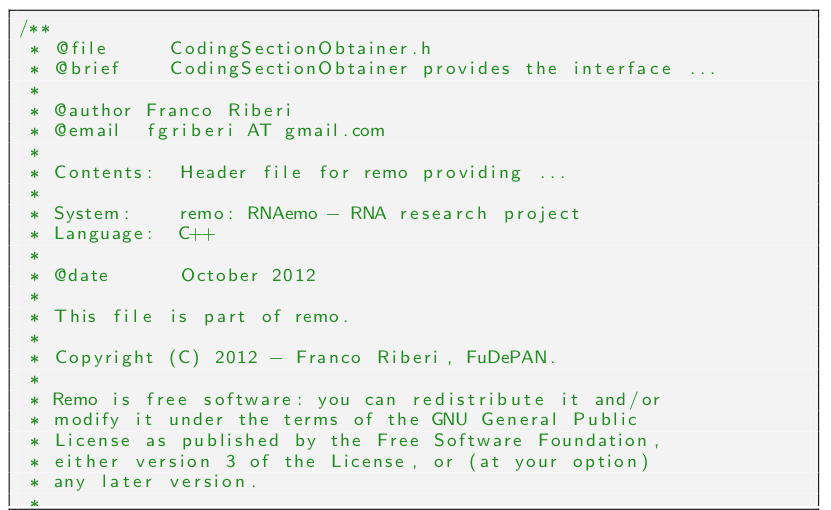
\includegraphics[scale=.35]{images/doxygen.png}
  \end{frame}   

\section{Conclusión}
      \begin{frame}\frametitle{\textbf{Resultados}}
        \begin{block}{Termodinámicos}
           \begin{itemize}
              \item \textit{Estructura Secundaria:} mayor cantidad de uniones GC en el humanizado que en el original. Mayor cantidad de stacks y más largos en el humanizado que en el original.

              \item \textit{$_m$$_i$RNA vs RNA$_m$:}$_m$$_i$RNA tienen una mayor capacidad de hibridar con los RNA humanizados que con los originales. 

            \end{itemize}                  
        \end{block}

        \begin{block}{Biológicos}
          \textbf{En los virus estudiados se pudo observar que existe un uso de codones divergente respecto de los del huésped humano.} En principio significaría una menor velocidad de síntesis proteica.
          Es decir, al virus le convendría usar los codones humanizados, pero sin embargo disminuye la cantidad de nucleotidos disponible para aparearse, los cuales estimulan la producción de interferón.
          %Desventaja: no tiene los codones opimos
          %ventaja: serviría para escapar al efecto del interferon

          %\par Surgieron además dos factores no contemplados en la biblografía (\emph{Futuros trabajos}).
        \end{block}
      \end{frame}    

      \begin{frame}\frametitle{\textbf{Conclusión}}
        \begin{block}{Profesional}
          \begin{itemize}
            \item Nuevos conceptos (SOLID, TMP)
            \item Profundización de conceptos 
            \item Exigencia en calidad y eficiencia
            \item Trabajo interdisciplinario como forma de aplicar los conocimientos científicos en la resolución concreta de problemas que afectan la calidad de vida de las personas.
          \end{itemize}
        \end{block}
        \begin{block}{Personal}
          \begin{itemize}
            \item Trabajo grupal
            \item Adaptación a un nuevo entorno de desarrollo
            \item Fuertes lazos humanos
          \end{itemize}
        \end{block}
      \end{frame}    

      \begin{frame}\frametitle{\textbf{Aportes}}
        \begin{itemize}
        \item A FuDePAN:
          \begin{itemize}
              \item R-emo: \url{r-emo.googlecode.com}.
              \item Fideo: \url{fideo.googlecode.com}.
              \item Acuoso: \url{acuoso.googlecode.com}.
              \item Etilico: \url{etilico.googlecode.com}.
              \item Otros: biopp(\url{biopp.googlecode.com}).
          \end{itemize}
        \vskip .2cm
        \item A la comunidad científica:
            \begin{itemize}                
                \item Análisis y la formalización del problema biológico.
                \item Solución computacional al problema.                
                \item Publicaciones (SAV 2012 - 3CAB2C). 
            \end{itemize}                 
         \vskip .2cm 
         \end{itemize}       
      \end{frame}    

      \begin{frame}\frametitle{\textbf{Trabajos Futuros}}
        \begin{block}{Futuros Desarrollos}
          \begin{itemize}
            \item Agregar nuevos backends para folding e hibridización en \emph{fideo}.
            \item Agregar nuevos backends para la humanización en \emph{acuoso}.
            \item Implementar un módulo de control de marco de lectura de las secuencias.
            \item \emph{Realizar el mismo estudia aplicado a proteínas.}
          \end{itemize} 
        \end{block}
        \begin{block}{Trabajos relacionados indirectamente}
          \begin{itemize}
            \item Pruebas de laboratorio.
            \item Refutación de las nuevas hipótesis.
          \end{itemize} 
        \end{block}
      \end{frame}    

\section{Bibliografía}
    \begin{frame}\frametitle{\textbf{Bibliografía I}}
  	\begin{thebibliography}{4}
		  \beamertemplatebookbibitems
        \bibitem{pag1} “Biología.”
        \newblock \emph{Curtis H., Sue Barnes N., Schnek A. \& Flores G. 2006} 

        \bibitem{pag2} “UNAFold: Software for Nucleic Acid Folding and Hybridization.”
        \newblock \emph{N.R. Markham \& M.Zuker. 2008} 
                
        \bibitem{pag3} “Thermodynamics of RNA-RNA Binding.”
        \newblock \emph{Muckstein et al. 2005}         

        \bibitem{pag4} “siRNA, miRNA and HIV: promises and challenges.”
        \newblock \emph{Man Lung YEUNG. 2005}         

        \bibitem{pag5} “RNA structural motifs : building blocks of a modular biomolecule.”
        \newblock \emph{D. K. Hendrix at el. 2006}         
		\end{thebibliography}
    \end{frame} 

    \begin{frame}\frametitle{\textbf{Bibliografía II}}
    \begin{thebibliography}{4}
      \beamertemplatebookbibitems      
        \bibitem{pag6} “Thermodynamics of RNA-RNA Interaction.”
        \newblock \emph{U. Muckstein \& H. Tafer. 2006}         

        \bibitem{pag7} “The extent of codon usage bias in human RNA viruses and its evolutionary origin.”
        \newblock \emph{Gareth M. Jenkins and Edward C. Holmes. 2003}         

        \bibitem{pag8} “Computational Methods for RNA Secondary Structure.”
        \newblock \emph{Zuker, Michael. 2006}         

        \bibitem{pag8} “Fast folding and comparison of RNA secondary structures.”
        \newblock \emph{Hofacker and at el. 1994}         
    \end{thebibliography}
    \end{frame}

    \begin{frame}\frametitle{\textbf{Bibliografía III}}
		\begin{thebibliography}{4}
		  \beamertemplatebookbibitems
		    \bibitem{pag9}“The C++ Programming Language, Third Edition.”
        \newblock \emph{Bjarne Stroustrup. Addison-Wesley. 1997} 

        \bibitem{pag10}“Object Design Roles, Responsibilities and Collaborations.”
        \newblock \emph{Rebeca Wirfs-Brock and Alan McKean. Addison-Wesley. 2002} 

        \bibitem{pag11}“Design Principles and Design Patterns.”
        \newblock \emph{Robert C. Martin. 2000} 
        
        \bibitem{pag12}“An Introduction to Software Architecture.”
        \newblock \emph{Garlan  && Shaw. Carnegie Mellon University. 1994} 

        \bibitem{pag13}A Framework for Small Distributed Projects and a Protein Clusterer Application.”
        \newblock \emph{Guillermo Biset. UNRC. 2009}         
		\end{thebibliography}
    \end{frame}

	\begin{frame}\frametitle{\textbf{Preguntas}}
			\begin{center}
				
\includegraphics[height=5cm]{images/preguntas.png}
			\end{center}
	\end{frame}	

\begin{frame}\frametitle{\textbf{Agradecimientos}}
\begin{center}
  \normalsize
  ``La vida sin pruebas y desafíos no sería provechosa, sino.  \\
  ¿Como aprenderíamos?"

  \begin{flushright}
  \textit{Josue Alvarez. Guatemala}\\
  \end{flushright}
   
  \pause   
  \vspace{1cm}
  %3\huge
  \textbf{Muchas Gracias \\ por su atención...!} 
\end{center}
\end{frame}

\end{document}